% ==============================================================================
% Tese Marcos A. Spalenza
% Capítulo 3 - Avaliação do Trabalho
% ==============================================================================
\chapter{Experimentos e Resultados}
\label{cap-experimentos}

O \textit{p}Nota é um sistema desenvolvido como laboratório para integrar melhorias na análise e avaliação de propostas de forma multidisciplinar, como discutido anteriormente. Para interagir com os usuários, o \textit{p}Nota se apoia em plataformas AVA na Universidade Federal do Espírito Santo (UFES). Nesse período, durante o desenvolvimento foram adicionadas diferentes técnicas para desenvolver a compreensão linguística e avaliativa do modelo SAG proposto. Os testes envolveram um conjunto de atividades com mais de 126 questões e 2805 respostas \cite{spalenza2016a}. Nesses testes foram analisadas formas distintas de escrita e em diferentes níveis de instrução, do Ensino Básico à Pós-Graduação, abordando tópicos distintos como Computação, Arquivologia, Ciências, Filosofia, Economia e Medicina. Entretanto, para avaliar o sistema é exposta aqui uma série de experimentos com \textit{datasets} encontrados na literatura.

Este capítulo apresenta os experimentos das duas etapas avaliativas. A primeira avalia a parte fundamental da técnica de \textit{Active Learning} do sistema \textit{p}Nota, com o uso da \textit{clusterização} para a identificação dos principais itens de resposta em cada base de dados. Na sequência, a segunda apresenta os métodos de classificação, a qualidade do aprendizado do sistema na predição de notas e a sua adequação ao modelo esperado pelo tutor.

\section{\textit{Datasets}}

De acordo com a literatura, foram selecionadas nove bases de dados, em português e inglês. Cada base de dados foi utilizada conforme sua disponibilidade e suas características. Alguns \textit{datasets} estão em linguagens que seria possível o processamento mas é necessário maior conhecimento da linguagem para adaptação ao \textit{p}Nota, como o \textit{JapaneseSAS} (japonês) \cite{ishioka2017}, \textit{Cairo University Dataset} (árabe) \cite{gomaa2019}, \textit{Corpus of Reading comprehension Exercises in German (CREG)} (alemão) \cite{ziai2012}, \textit{Science Answer Assessment (ScAA)} (hindi) \cite{agarwal2020} e o \textit{Chinese Educational Short Answers (CESA)} (chinês) \cite{ding2020}. Outros \textit{datasets} foram descartados pela indisponibilidade, como o \textit{Critical Reasoning for College Readiness (CR4CR) Assessment} \cite{condor2021}, o \textit{Cordillera Corpus} \cite{zhang2020}, entre outros inúmeros privados. Nesse caso enquadra-se grande quantidade de artigos, com coleta de dados local e sem acesso público. As nove bases de dados da literatura acessíveis foram organizadas por formato das notas atribuídas: ordinais, discretas e contínua \cite{morettin2010}. 

Em bases de dados com notas \textit{ordinais} o método avaliativo do tutor é dado de forma textual e categórica. A representação do rótulo não estabelece escalas para o sistema, não sendo possível mensurar a diferenças na escala \textit{a priori}. O modelo formado deve compreender as estruturas textuais de forma simbólica, caracterizando a essência de cada nível. Portanto, o classificador deve ser robusto para aprender a relevância das respostas pela equivalência de palavras-chave. Basicamente, é fundamental para o classificador produzir um modelo com as informações essenciais para a resposta receber tal categoria e reproduzir o modelo.

Por outro lado, outra situação acontece com bases de dados avaliadas com notas contínuas. As notas \textit{contínuas} não apresentam níveis, mas sim intervalos numéricos. As respostas recebem notas de acordo com o intervalo avaliativo. Apesar de numérico, o fato de a variável não definir uma categoria que represente a divergência entre respostas dificulta o aprendizado do modelo avaliativo. Ao sistema, isso torna subjetiva a expectativa de resposta. Assim, esse tipo de atividade é avaliado por interpolação. Nesse caso, o sistema realiza uma regressão de acordo com os pontos conhecidos, gerando a nota pela referência ao grau de similaridade para as demais respostas.

Por fim, a avaliação \textit{discreta} numérica é a mais comum. Esse modelo favorece também os sistemas computacionais na criação da representação de resposta por categoria de nota à medida que a categoria induz a equivalência de todas as respostas associadas. Assim, o sistema consegue mensurar equivalência e divergências pelos indícios de proximidade entre respostas avaliadas já conhecidas para além da mesma categoria. O desafio do sistema com esse tipo de nota é criar um bom modelo de classificação que aprenda essa relação dupla. Para além da categoria das respostas, o sistema passa a ter que interpretar as informações fundamentais de cada classe e a escala de divergência para as demais categorias. Na Tabela \ref{tab-datasets} cada \textit{dataset} é apresentado em detalhes, incluindo o número de questões, o total de respostas, o modelo avaliativo aplicado e a linguagem.

\begin{table}[!h]
\centering
\caption{Bases de dados e suas principais caracter{\'i}sticas.}
\label{tab-datasets}
\begin{tabular}{r |c c c c} 
 \hline
 Dataset & Quest{\~o}es & Respostas & Modelo Avaliativo & Linguagem \\ \hline
 SEMEVAL2013 Beetle & 47 & 4380 & ordinal & Ingl{\^e}s \\
 SEMEVAL2013 SciEntsBank & 143 & 5509 & ordinal & Ingl{\^e}s \\
 Kaggle ASAP-SAS & 10 & 17043 & discreto & Ingl{\^e}s \\
 Powergrading & 10 & 6980 & discreto & Ingl{\^e}s \\
 UK Open University & 20 & 23790 & discreto & Ingl{\^e}s \\
 University of North Texas & 87 & 2610 & cont{\'i}nuo & Ingl{\^e}s \\
 Kaggle PTASAG & 15 & 7473 & discreto & Portugu{\^e}s \\
 Projeto Feira Liter{\'a}ria & 10 & 700 & discreto & Portugu{\^e}s \\
 VestUFES & 5 & 460 & cont{\'i}nuo & Portugu{\^e}s \\
 \hline
 \hline
\end{tabular}
\end{table}

Na Tabela \ref{tab-datasets} são descritos os nove \textit{datasets} utilizados nos experimentos deste capítulo. Por meio das características apresentadas, é possível identificar uma regularidade interna de cada \textit{dataset}. Entretanto, entre os \textit{datasets} existe uma variação muito grande com questões de 30 até mais de 1800 respostas. É importante destacar ainda que, a definição de respostas curtas e as características textuais das respostas de cada um desses \textit{datasets} foi descrita no Capítulo \label{cap1-intro}, em especial na Tabela \ref{tab-features}. No total, esse \textit{corpora} contém 347 questões e 68.945 respostas. Cada base de dados e sua descrição completa são apresentadas a seguir:


\subsection{\textit{Dataset} \textit{Beetle} do \textit{SEMEVAL'2013 : Task 7} \textit{(Inglês)}}
\label{beetle-db}

\textit{Beetle} \cite{dzikovska2012} é um dos \textit{datasets} utilizados durante o \textit{International Workshop on Semantic Evaluation - SEMEVAL'2013}. O \textit{SEMEVAL} seleciona anualmente uma série de desafios em análise semântica e apresenta no formato de competição. O \textit{corpus Beetle} foi selecionado para a \textit{Task 7: The Joint Student Response Analysis and 8th Recognizing Textual Entailment Challenge} \cite{dzikovska2013}. Portanto, a competição consistia em duas propostas. A primeira é a análise e avaliação das respostas obtidas e a segunda o reconhecimento da relação textual entre as respostas coletadas e a expectativa de resposta do professor.

Esse \textit{dataset} consiste em uma coleção de interações entre estudantes e o sistema \textit{Beetle II}. Beetle II é um Sistema Tutor Inteligente (STI) para aprendizado de conhecimentos básicos em Eletricidade e Eletrônica do Ensino Médio. Os alunos foram acompanhados durante três a cinco horas para preparar materiais, construir e observar circuitos no simulador e interagir com o STI. Esse sistema apresenta as questões aos alunos, avalia as respostas e envia \textit{feedbacks} via \textit{chat}. Na construção desse \textit{dataset} foram acompanhados 73 estudantes voluntários da \textit{Southeastern University} dos Estados Unidos.

Foram aplicadas questões categorizadas em dois tipos: factuais e explicativas. As questões factuais requerem que o aluno nomeie diretamente determinados objetos ou propriedades. Enquanto isso, as questões explicativas demandam que o aluno desenvolva a resposta em uma ou duas frases. Para a formação do \textit{dataset} foram adicionadas apenas as atividades do segundo tipo, pois representam maior complexidade para sistemas computacionais. No total foram selecionadas 47 questões com 4380 respostas. A avaliação foi feita conforme o domínio demonstrado sobre o assunto em cinco categorias: \textit{correct}, \textit{partially-correct-incomplete}, \textit{contradictory}, \textit{irrelevant} e \textit{non-domain}. Durante a anotação o coeficiente \textit{Kappa} obtido foi de 69\% de concordância.


\subsection{\textit{Dataset} \textit{SciEntsBank} do \textit{SEMEVAL'2013 : Task 7} \textit{(Inglês)}}
\label{scientsbank-db}

O \textit{corpus Science Entailments Bank (SciEntsBank)} \cite{dzikovska2012} é um dos \textit{datasets} utilizados durante o \textit{International Workshop on Semantic Evaluation (SEMEVAL'2013)} \cite{dzikovska2013}, com foco na avaliação de sistemas conforme a sua capacidade de análise e exploração semântica da linguagem. É uma base de dados formada por questões da disciplina de ciências. Na avaliação 16 assuntos distintos são abordados entre ciências físicas, ciências da terra, ciências da vida, ciências do espaço, pensamento científico e tecnologia. 

As questões são parte da \textit{Berkeley Lawrence Hall of Science Assessing Science Knowledge (ASK)} com avaliações padronizadas de acordo com o material de apoio \textit{Full Option Science System (FOSS)}. Participaram estudantes dos Estados Unidos de terceira a sexta série, coletando em torno de 16 mil respostas. Porém, entre as questões de preenchimento, objetivas e discursivas, foram utilizadas apenas as discursivas, que requisitavam explicações dos alunos segundo o tema. As respostas foram graduadas em cinco notas ordinais: \textit{correct}, \textit{partially-correct-incomplete}, \textit{contradictory}, \textit{irrelevant} e \textit{non-domain}. O \textit{SciEntsBank}, então, consiste em um conjunto com 143 questões selecionadas e 5509 respostas. No processo de avaliação foi observado o coeficiente \textit{Kappa} com 72,8\% de concordância.

\begin{comment}
[('contradictory', 557), ('correct', 2241), ('irrelevant', 1248), ('non_domain', 26), ('partially_correct_incomplete', 1437)] 5509 SCIENTSBANK

[('contradictory', 1160), ('correct', 1841), ('irrelevant', 130), ('non_domain', 218), ('partially_correct_incomplete', 1031)] 4380 BEETLE 
\end{comment}

\subsection{\textit{Dataset} do Concurso ASAP-SAS no \textit{Kaggle} \textit{(Inglês)}}
\label{kaggle-db}

A origem da base de dados \textit{ASAP - SAS}, \textit{Automated Student Assessment Prize - Short Answer Scoring} é uma competição proposta pela \textit{Hewllet Foundation} na plataforma \textit{Kaggle}\footnote{The Hewlett Foundation - Short Answer Scoring: https://www.kaggle.com/c/asap-sas}. A competição consistiu em três fases:

\begin{itemize}
\item Fase 1:  Demonstração em respostas longas (redações); 
\item Fase 2:  Demonstração em respostas curtas (discursivas);
\item Fase 3:  Demonstração simbólica matemática/lógica (gráficos e diagramas).
\end{itemize}

Seu objetivo era descobrir novos sistemas de apoio ao desenvolvimento de escolas e professores. Especificamente, as três fases destacam a atividade lenta e de alto custo de avaliar manualmente testes, mesmo que com padrões bem definidos. Uma consequência disso é a redução do uso de questões discursivas nas escolas, dando preferência para as questões objetivas para evitar a sobrecarga de trabalho. Isso evidencia uma gradativa redução da capacidade dos professores em incentivar o pensamento crítico e as habilidades de escrita. Portanto, os sistemas de apoio, são uma possível solução para suportar os métodos de correção, avaliação e feedback ao conteúdo textual dos alunos.

Nesse contexto, a competição apresentou dez questões multidisciplinares, de ciências a artes. Estão distribuídas 17.043 respostas de alunos entre essas atividades. Para chegar a essa quantidade, foram selecionadas por volta de 1.700 respostas entre 3.000 respostas em cada atividade. Cada resposta tem aproximadamente 50 palavras. A primeira avaliação foi dada pelo primeiro especialista como nota final e a segunda nota foi atribuída apenas para demonstrar o nível de confiança da primeira nota. A avaliação apresentada por dois especialistas demonstrou concordância de 90\% no coeficiente \textit{Kappa}.


\subsection{\textit{Dataset} \textit{Powergrading} \textit{(Inglês)}}
\label{powergrading-db}
Elaborado com o \textit{United States Citizenship Exam} (USCIS) em 2012, a base de dados \textit{Powergrading} contém dez questões e 6980 respostas \cite{basu2013}. Desenvolvida originalmente para destacar a possibilidade de avaliação massiva, o \textit{dataset} selecionou 698 respostas para cada uma das questões. As respostas foram geradas com \textit{Amazon Mechanical Turk}, serviço remoto de análise manual de conteúdo para anotação da \textit{Amazon}. Foi coletada por um grupo de pesquisa da \textit{Microsoft}\footnote{Powergrading: https://www.microsoft.com/en-us/download/details.aspx?id=52397} e cada questão acompanha um modelo de resposta e as respostas recebidas para cada questão.  Além disso, acompanha o \textit{dataset} outras dez questões não avaliadas.

Foram requisitadas respostas com poucas palavras, atingindo no máximo uma ou duas sentenças. Por conta disso, os resultados são respostas muito curtas com quatro palavras em média. Em geral, por conta da convergência, vários padrões de resposta se repetem \cite{riordan2017}. Com avaliações binárias, 1 para resposta correta e 0 para incorreta, cada resposta apresenta avaliações de três diferentes tutores. Apesar de alguns trabalhos assumirem um dos avaliadores como padrão, foi utilizado como modelo de avaliação a resultante da comparação entre os três. Apesar de não ter complexidade linguística, ocorreu contradição entre os avaliadores em 470 respostas. Em valores percentuais, isso representa 7\% do total de respostas do conjunto de dados.

\begin{comment}
Respostas não coincidentes em cada questão
q1 - 1 q2 - 12 q3 - 145 q4 - 45 q5 - 18 q6 - 52 q7 - 20 q8 - 17 q13 - 108 q20 - 52
\end{comment}

\subsection{\textit{Dataset} da \textit{UK Open University} \textit{(Inglês)}}
\label{openunv-db}

A base de dados da \textit{UK Open University} é um conjunto de questões coletadas na disciplina de introdução a ciências, denominada \textit{S103 - Discovering Science} \cite{jordan2012}. O foco do conjunto de atividades são abordagens em questões factuais bem concisas, não excedendo 20 palavras. Os alunos receberam as atividades via ambiente virtual da \textit{Intelligent Assessment Technologies (IAT)}, o \textit{FreeText Author}. O \textit{FreeText Author} foi utilizado como um método de \textit{CAA} de modo interativo e com resultado automático analisando a resposta do aluno segundo os padrões de resposta conhecidos. O sistema permitiu uma sequência de envios e apresentava comentários da resposta como \textit{feedback} para os alunos. Dependendo da complexidade da resposta, o tempo de retorno dos resultados varia muito entre alguns poucos minutos até mais do que um dia.

O \textit{dataset} é de acesso privado, mas foi disponibilizado pelos autores para este estudo. Entre as suas 20 questões, esse \textit{dataset} apresenta diferentes quantidades de respostas entre 511 e 1897. A avaliação é discreta e binária, definindo cada resposta como correta ou incorreta. Não existem notas intermediárias, representando diretamente se o aluno atendeu ou não os requisitos da resposta. 


\subsection{\textit{Dataset} da \textit{University of North Texas} \textit{(Inglês)}}
\label{ntexasunv-db}

O \textit{dataset} da \textit{University of North Texas - UNT} \cite{mohler2011}, conhecido como \textit{Texas dataset}\footnote{Texas Dataset: https://web.eecs.umich.edu/{\textasciitilde}mihalcea/downloads.html}, é uma coleção de questões discursivas extraída no curso de Ciência da Computação. Composto por 80 atividades únicas, esse conjunto contempla dez listas de exercícios com até sete questões e dois testes com dez questões cada. Foram aplicados em um ambiente virtual de aprendizagem durante a disciplina de Estrutura de Dados para 31 alunos. No total o \textit{dataset} é composto por 2.273 respostas de alunos entre as 80 atividades.

A avaliação foi feita com cinco notas discretas, de 5 equivalente a resposta perfeita até 0 completamente incorreta. Foram avaliadas por dois avaliadores independentes, estudantes do curso de Ciência da Computação. Para os autores, o modelo seguido pelo sistema deve ser a resultante da média ente os avaliadores, em intervalo contínuo. Entre as notas atribuídas, 57,7\% das respostas receberam a mesma pontuação. Enquanto isso, um nível de diferença entre as notas representou 22,9\% do total de respostas. Foi constatado também que, dentre as diferenças na avaliação, o avaliador 1 atribuía notas maiores notas 76\% das vezes.

\subsection{\textit{Dataset} \textit{PTASAG} no \textit{Kaggle} \textit{(Português)}}
\label{ptasag-db}

A \textit{PTASAG - Portuguese Automatic Short Answer Grading Data} é uma base de dados brasileira apresentada por \cite{galhardi2018b} e disponibilizada na plataforma \textit{Kaggle}\footnote{PT-ASAG-2018: https://www.kaggle.com/lucasbgalhardi/pt-asag-2018}. Foi coletada pela Universidade Federal do Pampa - Unipampa em conjunto com cinco professores de biologia do Ensino Fundamental. Foram criadas 15 atividades com base no sistema Auto-Avaliador CIR. Em biologia, os tópicos abordados foram sobre o corpo humano. Cada questão acompanha uma lista de conceitos, as respostas avaliadas e as respostas candidatas criadas pelos professores como referência. Foram criadas entre duas e quatro respostas candidatas contendo entre três e seis palavras-chave.

As atividades foram aplicadas no Ensino Fundamental para 326 estudantes de 12 a 14 anos do 8\textsuperscript{\b{o}} e do 9\textsuperscript{\b{o}} ano. Também foram aplicadas a 333 alunos do Ensino Médio de 14 a 17 anos. As respostas foram avaliadas por 14 estudantes de uma turma do último ano, considerando uma escala de notas de 0 a 3:

\begin{itemize}
\item Nota 0: Majoritariamente incorreta, fora de tópico ou sem sentido;
\item Nota 1: Incorreta ou incompleta mas com trechos corretos;
\item Nota 2: Correta mas com importantes trechos faltantes;
\item Nota 3: Majoritariamente correta apresentando os principais pontos.
\end{itemize}

No total, participaram 659 estudantes com um total de 7.473 respostas. Cada uma das 15 questões apresenta entre 348 e 615 respostas. Apenas quatro questões foram examinadas por mais de um avaliador para verificar a concordância entre eles. O coefficiente \textit{Kappa} observado foi de, em média, 53.25\%.


\subsection{\textit{Dataset} do Projeto Feira Literária das Ciências Exatas \textit{(Português)}}
\label{findes-db}

É um conjunto de dados coletados durante o Projeto Feira Literária das Ciências Exatas \cite{nascimento2020}. As questões foram obtidas durante uma Atividade Experimental Problematizada por meio de um livro paradidático, ou seja, cujo objetivo primário não é o apoio didático. O livro escolhido foi \textit{A Fórmula Secreta} de David Shephard. 

Conforme o livro, os professores formularam dez atividades e ministraram para 70 alunos do 5º ano de Ensino Fundamental. Essas atividades ministradas descreviam situações práticas de química básica. No total, o conjunto de dados conta com dez questões, 700 respostas e suas respectivas avaliações.


\subsection{\textit{Dataset} do Vestibular UFES \textit{(Português)}}
\label{vest-ufes-db}

A base de dados VestUFES \cite{pissinati2014} é uma amostra das questões discursivas de Português do vestibular da UFES em 2012. A amostra selecionada contém 460 respostas divididas igualmente entre as cinco questões de língua portuguesa, também referentes a respostas dadas por 92 diferentes alunos.

Cada resposta foi avaliada por dois avaliadores. De acordo com o vestibular da universidade, os avaliadores atribuíram notas entre 0 e 2 pontos em cada questão, totalizando 10 na soma da prova. Caso houvesse divergências de mais de 1 ponto entre as correções um terceiro avaliador era acionado para reavaliar a coerência das notas. A nota das respostas do \textit{dataset} foram redimensionadas pelo autor para o intervalo de 0 a 10 pontos. Na nova escala, as diferenças observadas entre os avaliadores foi de, em média, 1,38 ponto com desvio padrão de 1,75.


\begin{comment}
\subsection{Dataset das Disciplinas UFES \textit{(Português)} \label{disciplinas-ufes-db}
Essa base de dados foi coletada de algumas disciplinas ministradas na Universidade Federal do Espírito Santo - UFES entre 2015 e 2016 através do Moodle do Laboratório Computação de Alto Desempenho - LCAD. Entre as disciplinas estão Metodologia e Técnicas de Pesquisa Científica, Filosofia e Tecnologia da Informação II. Totalizando 45 atividades, neste \textit{dataset} foram recebidas 1162 submissões com média 25,82 e desvio padrão de 13,54 respostas por atividade.

O diferencial dessa base de dados é a mudança de características nas respostas encontradas nas múltiplas disciplinas, professores e alunos. Observam-se alterações consideráveis quanto ao tamanho, número de grupos, critério avaliativo ou objetividade. 
\end{comment}


\section{Experimentos}
\label{sec-experimentos}

Os experimentos realizados têm como intuito demonstrar a qualidade do método proposto de \textit{Active Learning}, com otimização do esforço de anotação humano. Assim, é esperada uma boa forma na amostragem tal qual o ganho de desempenho nos resultados de classificação. Com os \textit{datasets} conhecidos da literatura, é possível comparar nossa proposta de análise das estruturas textuais em relação aos principais trabalhos publicados. Inicialmente, os experimentos mostram o desempenho da etapa de \textit{clusterização} com a caracterização dos \textit{clusters} formados. Essa etapa indica a qualidade da amostragem em relação ao objetivo da atribuição de notas. Na sequência, apresentam-se comparativos com os classificadores da literatura, tentando maximizar os resultados obtidos com qualidade compatível aos demais trabalhos.


\subsection{Resultados de \textit{Clusterização}}
\label{sec-res-clustering}

Nessa primeira análise, observa-se a qualidade dos \textit{clusters} formados. Assim, é investigado se a forma utilizada para construção dos \textit{clusters} foi efetiva para formação das amostras. Nessa etapa é essencial que a amostragem colete toda a diversidade de notas, adquirindo conhecimento que torna possível comparar os níveis de nota. Neste identificam-se as regiões que estabelecem diferenças entre contextos, com identificação de equivalências e divergências, isolando \textit{outliers}. Assim, essa primeira etapa é definitiva para a qualidade do aprendizado via \textit{Active Learning}.

A formação dos \textit{clusters} foi feita com base em uma otimização do \textit{elbow method}, caracterizando a dispersão das amostras \cite{spalenza2019}. Os resultados obtidos, visam ter \textit{clusters} mais homogêneos, segundo os índices de validação. O índice utilizado foi o CVS, avaliando o coeficiente de variação do tamanho dos \textit{clusters} formados e evitando grande concentração. Os múltiplos contextos e a sobreposição entre as notas atribuídas são detalhes observados em grandes \textit{clusters}. Na avaliação dos clusters, utilizam-se as métricas CA, HS e CS, descritas na Seção \ref{subsec-clusterizacao}. Os resultados obtidos em cada um dos \textit{datasets} é apresentado na Tabela \ref{tab-clstr-index}.

\begin{table}[!h]
\centering
\caption{Bases de dados e índices qualitativos de \textit{clusterização}.}
\label{tab-clstr-index}
\begin{tabular}{r | r r r }
\hline
    \textit{Dataset}  & CA & HS & CS \\ \hline 
    SEMEVAL2013 Beetle & 0,5897 & 0,2895 & 0,1856 \\
    SEMEVAL2013 SciEntsBank & 0,6064 & 0,2357 & 0,1789 \\
    UK Open University  & 0,7628 & 0,2825 & 0,0667 \\
    Projeto Feira Liter{\'a}ria & 0,6414 & 0,3920 & 0,2574 \\
    Kaggle ASAP-SAS  & 0,5364 & 0,1065 & 0,0741 \\
    Powergrading & 0,9032 & 0,6773 & 0,0760 \\
    Kaggle PTASAG  & 0,5208 & 0,2282 & 0,1418 \\
    University of North Texas & - & - & - \\
    VestUFES & - & - & - \\
\hline
\hline
\end{tabular}
\end{table}

Na Tabela \ref{tab-clstr-index} é mostrado um alto índice de relação entre \textit{clusters} e itens que receberam uma mesma nota. Isso implica em um CA médio de 65,15\%, atingindo até 90,32\% no \textit{dataset} \textit{Powergrading}. O CA, via voto majoritário, indica quantas amostras compartilham \textit{clusters} com diferentes avaliações. Pela atribuição de notas contínuas, os \textit{datasets} \textit{University of North Texas} e \textit{VestUFES} foram desconsiderados nessa análise.

É um dos objetivos da etapa de \textit{clusterização} que os grupos formados representem os tópicos abordados na questão. Assim, com efeito descritivo sobre os vínculos entre os \textit{cluster} e as notas, o CA indica o nível de complexidade para o reconhecimento de padrões e avaliação. No entanto, os índices HS e CS apontam a conexão entre cada classe de nota com os \textit{clusters} formados. Esses dois índices refletem algumas características dos problemas textuais.

O primeiro indica o nível de homogeneidade, ou seja, o percentual de \textit{clusters} formados por uma mesma nota. Estabelecer essa separabilidade entre classes e \textit{clusters} é uma tarefa muito complexa. Em especial na análise textual, é comum que as avaliações distintas ocorram em respostas com algum nível de sobreposição de termos. Ou seja, notas distintas podem apresentar algum nível de similaridade e formar um mesmo \textit{cluster}. Já o segundo indica a equivalência entre os \textit{clusters} formados e cada uma das instâncias de nota. No entanto, dada a liberdade textual, dificilmente as respostas que recebem uma mesma nota apresentam os mesmos termos como referência.

Desse modo, \textit{datasets} com classificação binária tendem a ter alto desempenho na \textit{clusterização}, como o \textit{Powergrading}. Porém, com muitos níveis de nota e textos maiores, \textit{datasets} como \textit{ASAP-SAS} e \textit{PTASAG}, tornam-se muito complexos para essa primeira etapa. O desempenho antes da etapa de amostragem mostra a eficiência dos classificadores para levar \textit{clusters} com divergências para uma melhoria considerável de desempenho. O desempenho das classificações após a amostragem é apresentado em detalhes na Seção \ref{sec-res-classificacao}. Para mostrar como os \textit{clusters} são formados por diferentes contextos, analisa-se também a similaridade entre centroides, indicando nessa etapa de \textit{Active Learning} que a \textit{clusterização} regionaliza as respostas segundo a interpretação dos contextos. Na Figura \ref{fig-hmPowergrading} é exposto o grau de similaridade encontrado nos \textit{clusters} formados para o \textit{dataset} \textit{Powergrading}.

\begin{figure}[!h]
\begin{minipage}[t]{.45\textwidth}
\centering
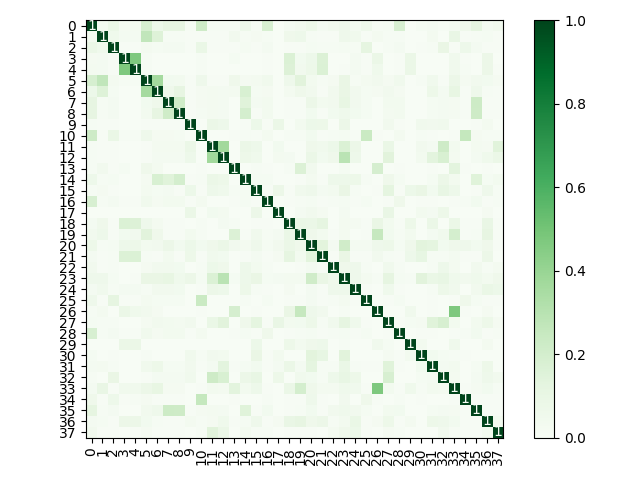
\includegraphics[width=\textwidth]{figuras/Powergrading/hm-q1.png} 
\subcaption{Atividade q1}
\end{minipage}%
\begin{minipage}[t]{.45\textwidth}
\centering
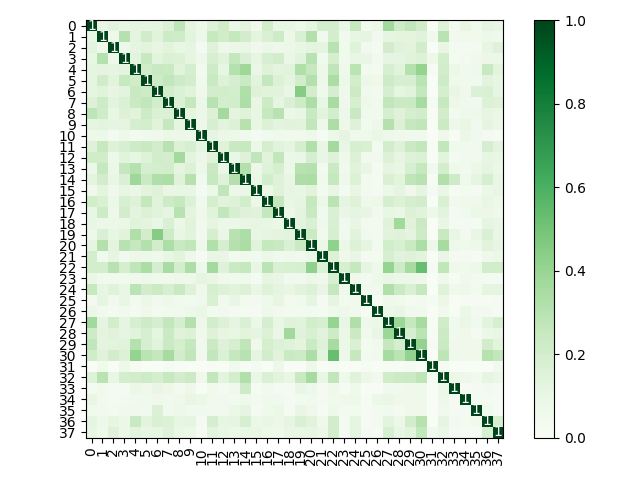
\includegraphics[width=\textwidth]{figuras/Powergrading/hm-q3.png} 
\subcaption{Atividade q3}
\end{minipage}%
\hfill
\begin{minipage}[t]{.45\textwidth}
\centering
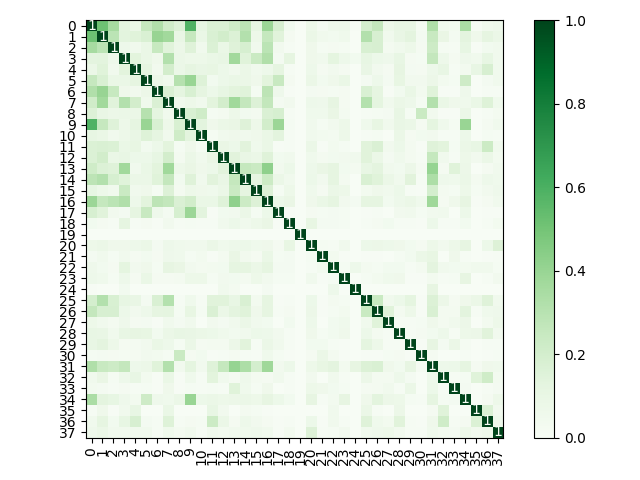
\includegraphics[width=\textwidth]{figuras/Powergrading/hm-q6.png} 
\subcaption{Atividade q6}
\end{minipage}%
\begin{minipage}[t]{.45\textwidth}
\centering
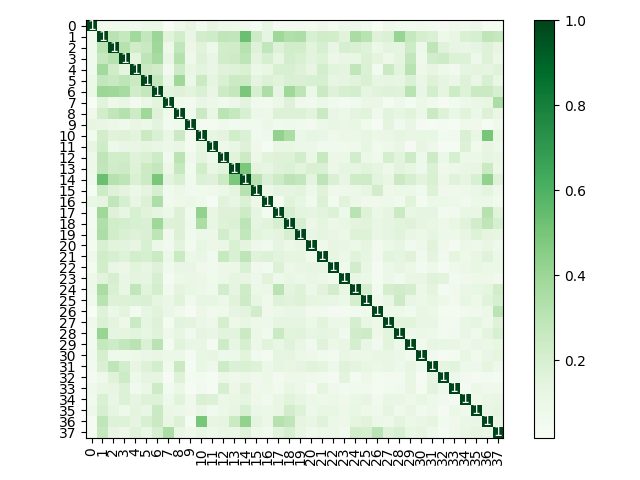
\includegraphics[width=\textwidth]{figuras/Powergrading/hm-q7.png} 
\subcaption{Atividade q7}
\end{minipage}
\caption{Similaridade entre \textit{centroides} para as atividades \textit{q1}, \textit{q3} e \textit{q6} e \textit{q7} em \textit{Powergrading}.}
\label{fig-hmPowergrading}
\end{figure}

Como pode ser observado na Figura \ref{fig-hmPowergrading}, os grupos de respostas formados são muito consistentes, sendo dissimilares em relação aos demais \textit{clusters}. Há nesses casos uma divergência do item médio (\textit{centroide}) do \textit{cluster} em relação aos demais grupos.  São denominados agrupamentos consistentes aqueles que todas as respostas têm um mesmo alinhamento, recebendo posteriormente uma mesma classe de nota. A atividade \textit{q1}, por exemplo, apresenta similaridade média de apenas 0,0355. Mesmo a que apresenta \textit{clusters} mais próximos, a atividade \textit{q7} apresenta em média 0,1387 de similaridade. As outras duas em destaque, atividades \textit{q3} e \textit{q6}, atingem 0,1207 e 0,0730. Assim, a etapa de \textit{clustering} têm potencial de formar zonas de equivalência e divergência com alta qualidade para as etapas de atribuição de notas. Essa alta qualidade indica \textit{clusters} bem separados de acordo com o contexto. A Figura \ref{fig-hmSciEntsBank} apresenta um caso oposto com a diferença entre os \textit{centroides} dos \textit{clusters} para a atividade \textit{SciEntsBank}.

\begin{figure}[!h]
\begin{minipage}[t]{.45\textwidth}
\centering
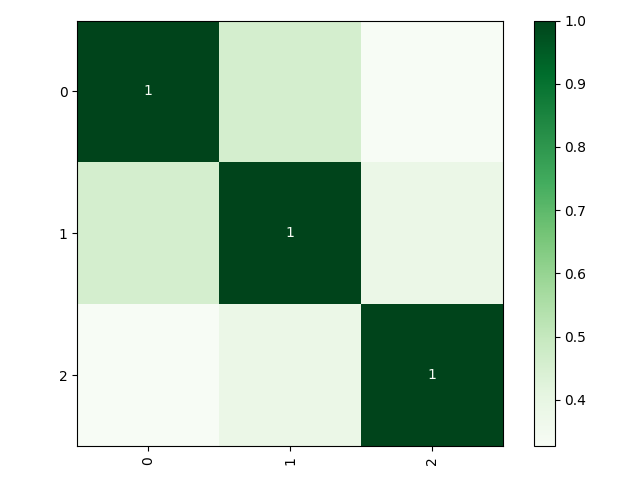
\includegraphics[width=\textwidth]{figuras/seb/hm-EM16b.png} 
\subcaption{Atividade EM16b}
\end{minipage}%
\begin{minipage}[t]{.45\textwidth}
\centering
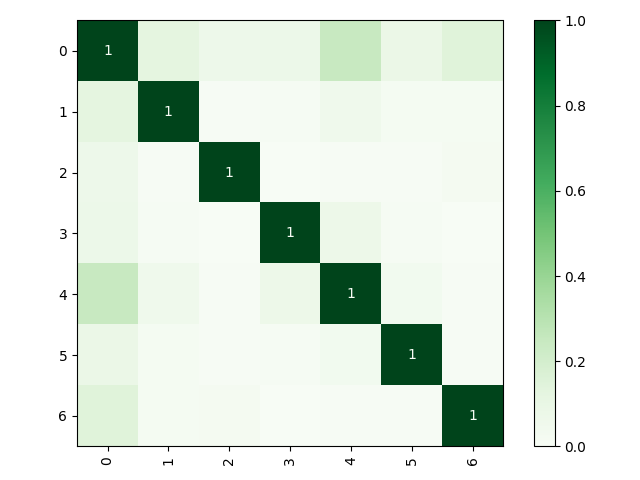
\includegraphics[width=\textwidth]{figuras/seb/hm-EM21b.png}
\subcaption{Atividade EM21b}
\end{minipage}%
\hfill
\begin{minipage}[t]{.45\textwidth}
\centering
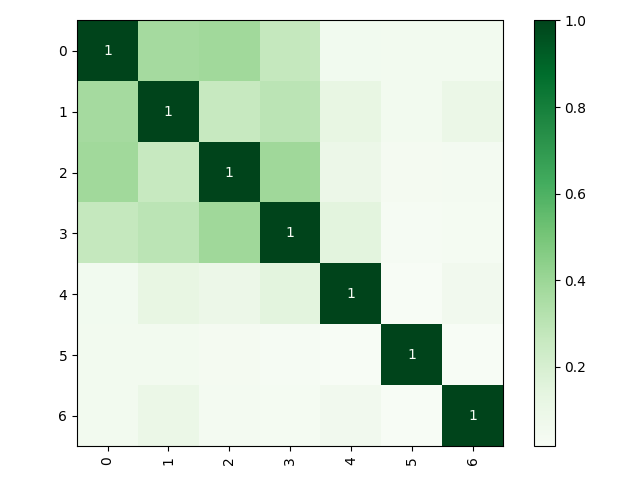
\includegraphics[width=\textwidth]{figuras/seb/hm-EM27b.png} 
\subcaption{Atividade EM27b}
\end{minipage}%
\begin{minipage}[t]{.45\textwidth}
\centering
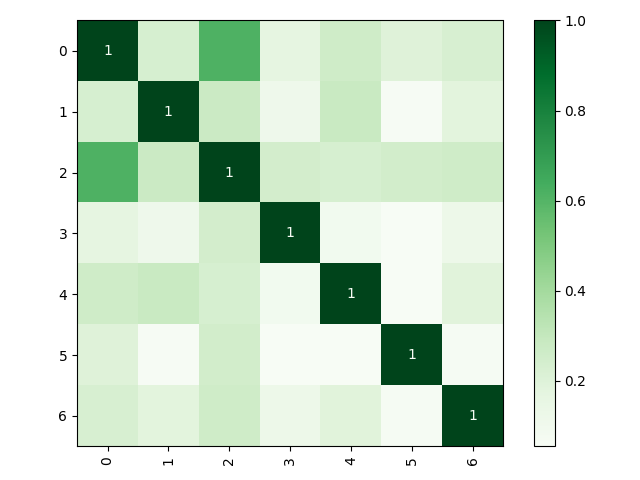
\includegraphics[width=\textwidth]{figuras/seb/hm-MX16a.png} 
\subcaption{Atividade MX16a}
\end{minipage}
\caption{Similaridade entre \textit{centroides} para as atividades \textit{EM16b}, \textit{EM21b}, \textit{EM27b} e \textit{MX16a} em \textit{SciEntsBank}.}
\label{fig-hmSciEntsBank}
\end{figure}

Como ilustrado na Figura \ref{fig-hmSciEntsBank}, há um resultado mais complexo de \textit{clusterização}, em especial, com poucas amostras. Diferentemente do que foi notado na questão anterior, existem situações distintas dentro de um mesmo \textit{dataset}. A primeira atividade \textit{EM16b} apresenta poucos \textit{clusters} e similaridade média de 0,3880. A segunda atividade \textit{EM21b} mostra uma boa separabilidade entre os dados com média de 0,0476 e máxima de 0,2442. A terceira atividade \textit{EM27b} mostra uma concentração entre alguns \textit{clusters}, com um núcleo de \textit{centroides} similares e outra parte bem distante, com similaridade média de 0,1361 e máxima entre \textit{centroides} de 0,3256. Por fim, a quarta atividade \textit{MX16a} mostra alguns \textit{clusters} muito próximos atingindo similaridade máxima de 0,6125 sendo a média entre \textit{centroides} de 0,1974.

Pelo índice de similaridade parcial ou total dos clusters formados pode-se considerar que algumas atividades mostram diferentes perspectivas de uma mesma classe ou mesclando diferentes classes. Assim, a identificação de padrões entre esses grupos de alta similaridade depende de um bom reconhecimento de padrões \textit{a posteriori}. Assim, é compreensível que os níveis de CA desses \textit{clusters} sejam baixos. No entanto, é importante obter ganhos na etapa de classificação, elevando o nível dos resultados alcançados.

\subsection{Resultados de \textit{Classificação}}
\label{sec-res-classificacao}

Após os resultados obtidos na etapa de \textit{clusterização}, é realizada a análise de classificação. Nesta, usam-se os classificadores tradicionais para avaliar o ganho em desempenho proporcionado pela etapa de \textit{Active Learning}. Tais experimentos, diferentemente do descrito para estudo dos \textit{clusters} formados, caracterizam-se pela simetria com  os artigos da literatura e os desafios da área. Como os \textit{datasets}, geralmente vêm particionados, foram agrupados os conjuntos de treino e teste para que a nosso método \textit{não-supervisionado} realize os particionamentos, preservando os percentuais.

Neste estudo, cada atividade foi processada isoladamente, distinguindo assim de alguns estudos que utilizam todas as atividades durante o treinamento. Essa técnica é comum em abordagens que precisam de maior quantidade de amostras para aprendizado. No entanto, proporcionalmente, ainda é necessário garantir a coesão do \textit{dataset} com o tema. Nesse caso, com o volume de dados ainda reduzido, os sistemas tornam-se específicos para um contexto. Além disso, em caráter multidisciplinar, a tendência é o sistema receber blocos distintos de atividades, cada qual em um contexto.

Outro fator comum encontrado na literatura é a adoção de métricas distintas na avaliação dos modelos. Os principais exemplos incluem métricas diretamente relacionadas com os testes e o grupo de amostras. Assim, são comuns os casos que a avaliação não leve em conta os problemas de desbalanceamento e a paridade entre experimentos. Em boa parte dos casos dos SAGs é reportado apenas o coeficiente \textit{Kappa} ou correlação de \textit{Pearson}. O \textit{Kappa} é considerada uma métrica robusta, que representa detalhes por categoria e a relação de avaliação \cite{bendavid2008}. Entretanto, individualmente, a escolha de uma métrica como essa indica apenas uma visão unilateral do problema \cite{delgado2019}. Uma consequência da aplicação de \textit{Active Learning} é o aprendizado gradual dos níveis de nota, conforme as iterações avaliativas e o ganho de informação. Durante cada ciclo o modelo busca se adaptar da melhor forma à diversidade de notas. De fato, com a integração humano-computador no processo avaliativo, é importante atentar-se na prevalência dos resultados de classificação, intra-classe e inter-classes de nota. 

Adicionalmente, ressalta-se o modelo de amostragem observado nos trabalhos da literatura. O percentual de amostragem foi aplicado de acordo com o conjunto de dados e os demais trabalhos, variando entre 70\% e 90\% das respostas. O alto percentual é comum pois é possível reaproveitar o treinamento para aplicar em novas amostras. Após o primeiro treinamento, apenas algumas intervenções do professor são necessárias para correção. Desta forma, gradativamente o esforço do professor pode ser minimizado. Nesses casos, principalmente com o \textit{p}Nota, com novos grupos de dados para cada atividade tornam-se necessárias apenas eventuais avaliações assimilar novos tópicos.

Seguindo a característica da avaliação, serão apresentados os resultados obtidos segundo a forma avaliativa adotada pelos professores. Os conjuntos de dados \textit{Beetle} e \textit{SciEntsBank} podem ser considerados mais complexos pela baixa quantidade de amostras para um modelo de avaliação de cinco categorias textuais (ordinais). Nestes \textit{datasets} do evento \textit{SEMEVAL' 2013}, foram apresentados três níveis de desafios. O primeiro nível é a avaliação de respostas não conhecidas, selecionadas aleatoriamente no conjunto de respostas (\textit{Unseen Answers}). O segundo nível compreende a correção de respostas em questões desconhecidas, ainda em um determinado domínio (\textit{Unseen Questions}). E, por fim, o terceiro nível está relacionado à análise de respostas em um domínio desconhecido (\textit{Unseen Domain}). Assim como a maioria dos sistemas SAG, o desafio que se enquadra no tópico aqui abordado é apenas o primeiro (\textit{Unseen Answers}), avaliando conjuntos de respostas dentro do tópico. 

Sendo a principal característica deste \textit{dataset} o desbalanceamento das classes \cite{dzikovska2013}, ambos os \textit{datasets} foram anotados em níveis de nota: \textit{correct}, \textit{partially-correct-incomplete}, \textit{contradictory}, \textit{irrelevant} e \textit{non-domain}. Evidencia-se pela complexidade, inclusive semântica, de separar as três categorias inferiores, \textit{contradictory}, \textit{irrelevant} e \textit{non-domain}. Utilizando os seis classificadores descritos na Seção \ref{subsec-classificacao}, são apresentados os resultados obtidos na Tabela \ref{tab-SEMEVAL}.

\begin{table}
\centering
\caption{Resultados dos seis classificadores testados nos \textit{datasets} do \textit{SEMEVAL' 2013}.}
\label{tab-SEMEVAL}
\begin{tabular}{l r r r r r}
    \hline
    \multicolumn{4}{l}{\textbf{Beetle}} &  \multicolumn{2}{r}{(5 Categorias)} \\ \hline
    & \multicolumn{5}{c}{M{\'e}tricas} \\ \cline{2-6}

     & ACC & PRE & REC & F1(m) & F1(w) \\ \cline{2-6}
    DTR & 61,90\% & 41,14\% & 43,08\% & 40,82\% & 60,01\% \\
    GBC & \textbf{62,32\%} & \textbf{41,63\%} & \textbf{43,66\%} & \textbf{41,25\%} & \textbf{60,06\%} \\
    KNN & 59,80\% & 35,98\% & 39,21\% & 36,38\% & 56,26\% \\
    RDF & 60,67\% & 39,21\% & 40,65\% & 38,67\% & 58,35\% \\
    SVM & 60,06\% & 36,86\% & 42,56\% & 38,10\% & 54,70\% \\
    WSD & 60,76\% & 37,28\% & 40,40\% & 37,59\% & 56,95\% \\

    \hline
    \\
    \\
    \hline
    \multicolumn{4}{l}{\textbf{SciEntsBank}} &  \multicolumn{2}{r}{(5 Categorias)} \\ \hline
     & \multicolumn{5}{c}{M{\'e}tricas} \\ \cline{2-6}

     & ACC & PRE & REC & F1(m) & F1(w) \\ \cline{2-6}
    DTR & 48,79\% & 38,94\% & 39,30\% & 38,01\% & 39,30\% \\
    GBC & \textbf{50,62\%} & \textbf{40,43\%} & 42,50\% & \textbf{39,93\%} & \textbf{49,04\%} \\
    KNN & 43,16\% & 34,88\% & 36,13\% & 33,89\% & 41,86\% \\
    RDF & 49,49\% & 37,84\% & \textbf{43,25\%} & 38,96\% & 45,67\% \\
    SVM & 46,51\% & 32,89\% & 41,01\% & 35,31\% & 40,45\% \\
    WSD & 47,43\% & 36,45\% & 40,21\% & 36,97\% & 44,43\% \\
    \hline
    \hline
\end{tabular}
\end{table}

Na Tabela \ref{tab-SEMEVAL} é mostrado o desempenho do sistema com os seis classificadores testados. Fica evidente que a performance do sistema é superior no \textit{Beetle} em relação ao \textit{SciEntsBank}. No \textit{dataset} \textit{Beetle} o melhor resultado obtido foi com o GBC, com ACC médio de 62,32\% e F1-ponderado de 60,06\%. No entanto, a diferença foi bem pequena em relação aos demais classificadores. No \textit{dataset} \textit{SciEntsBank} o resultado foi diferente, com o GBC apresentando resultados bem superiores em relação a alguns classificadores, com ACC médio de 50,62\% e F1-ponderado de 49,04\%. O KNN apresentou baixo desempenho, com ACC de apenas 43,16\%, devido aos vários níveis de nota entre as poucas respostas. Foram comparados os resultados obtidos no \textit{dataset} \textit{Beetle} na Figura \ref{fig-semeval-beetle}.

\begin{figure}[!h]
\centering
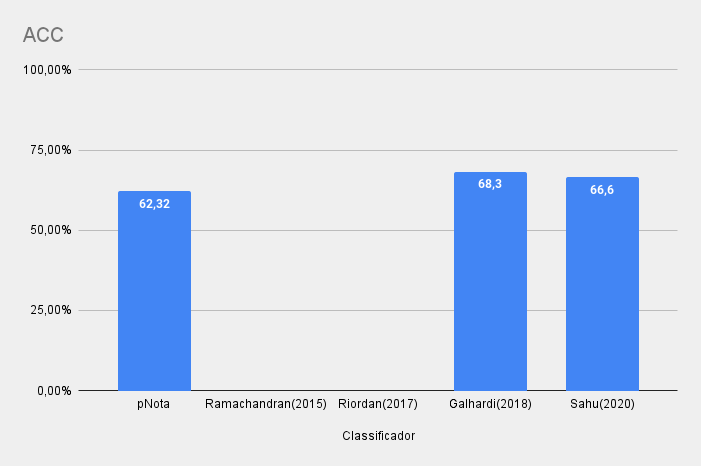
\includegraphics[width=.6\textwidth]{figuras/beetle/res-beetle-acc.png}
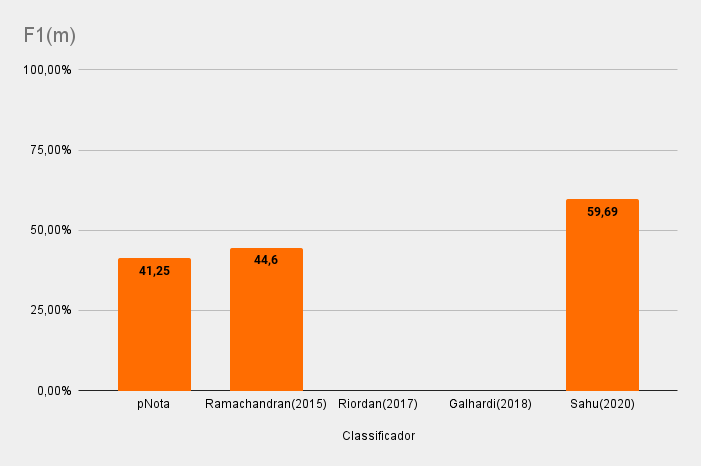
\includegraphics[width=.6\textwidth]{figuras/beetle/res-beetle-mfs.png}
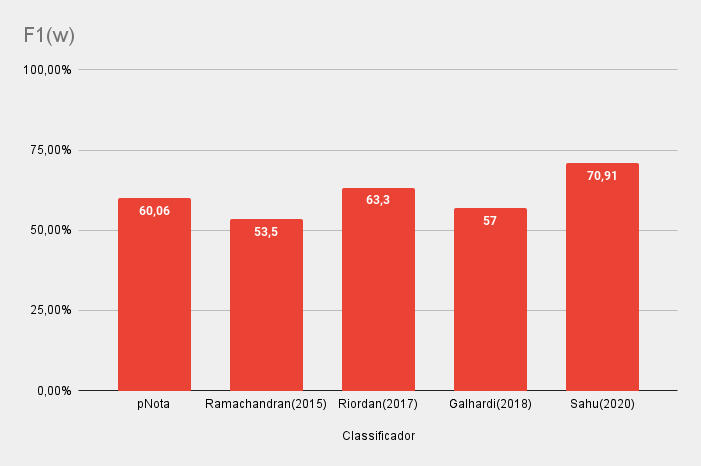
\includegraphics[width=.6\textwidth]{figuras/beetle/res-beetle-wfs.png}
\caption{Resultados obtidos no \textit{dataset} \textit{Beetle}.}
\label{fig-semeval-beetle}
\end{figure}


Na Figura \ref{fig-semeval-beetle}, é mostrado o desempenho do \textit{p}Nota e dos trabalhos da literatura em ACC, F1-macro e F1-ponderado. O melhor resultado encontrado na literatura foi apresentado por \cite{sahu2020}, com uma estratégia que realiza a combinação de vários níveis da estrutura textual, atingindo ACC de 66,6\% e F1-ponderado de 70,91\%. Neste, os autores incluem \textit{features} de similaridade semântica, de sobreposição léxica, de recuperação da informação, de similaridade de tópicos, similaridade entre \textit{feedbacks} e de alinhamento textual. Portanto, temos uma ampla aquisição de informação, combinando os métodos tradicionais \textit{Latent Semantic Analysis} (LSA), \textit{word embeddings}, \textit{Recall Oriented Understudy for Gisting Evaluation} (ROUGE), \textit{TF-IDF}, \textit{LDA}, dentre outros. A avaliação é dada posteriormente com \textit{ensembles} usando \textit{Random-Forest}.

No estudo realizado por \cite{galhardi2018c} encontra-se também uma combinação de \textit{features} que incluem estatísticas textuais, como o cálculo de erros, tamanhos de resposta e contagem de palavras por sentença. Essas estruturas eram comuns nos primeiros trabalhos da área, hoje avançando com análise da linguagem \cite{burrows2015}. Usando \textit{Random Forests} e \textit{Extreme Gradient Boosting} os autores alcançaram ACC de 68,3\% e F1-ponderado de 57\%. Um terceiro destaque vale para o trabalho de \cite{riordan2017}, com F1-ponderado de 63,3\%. Nesse caso, os autores não divulgaram as demais métricas. O resultado foi alcançado combinando \textit{word-embeddings}, \textit{Convolutional Neural Networks} (CNN) e \textit{Long Short-Term Memory} (LSTM). As notas são dadas no \textit{layer} de agregação por um modelo linear. Outra técnica aplicada é a sumarização, avaliando as respostas ao mensurar a similaridade dos grafos textuais \cite{ramachandran2015a, ramachandran2015b}. Essa estratégia ainda depende de combinar vários trechos da atividade, desde o enunciado até o quadro de \textit{rubrics}. De forma geral, os resultados obtidos no \textit{Beetle} são bem próximos entre eles. O desempenho intermediário indica o desafio de compreender as cinco categorias do \textit{dataset}. Outra perspectiva é dada nos resultados do \textit{SciEntsBank}, apresentados na Figura \ref{fig-semeval-seb}.

\begin{figure}[!h]
\centering
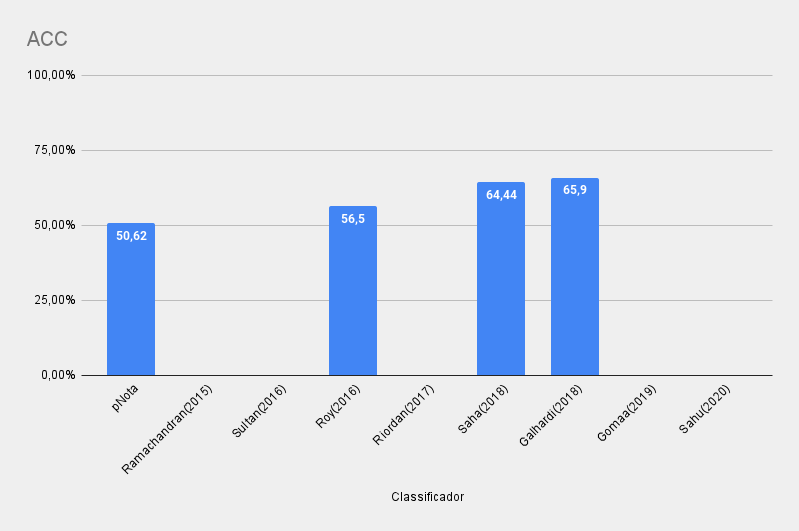
\includegraphics[width=.6\textwidth]{figuras/seb/res-seb-acc.png}
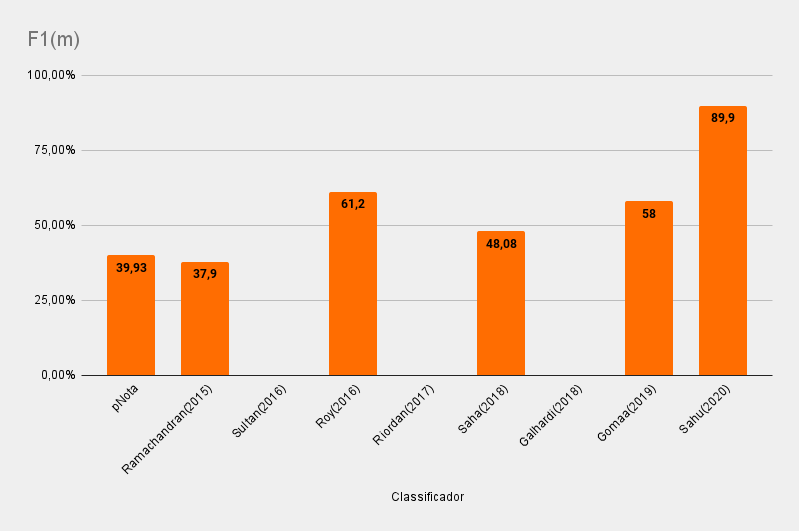
\includegraphics[width=.6\textwidth]{figuras/seb/res-seb-mfs.png}
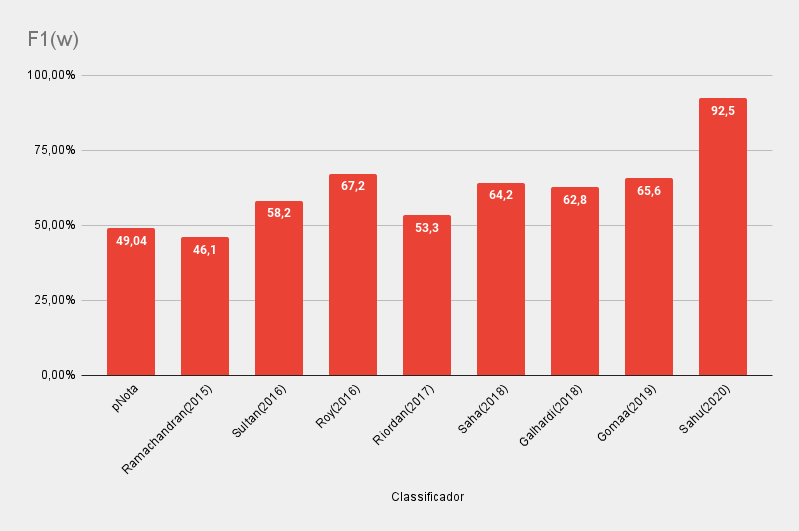
\includegraphics[width=.6\textwidth]{figuras/seb/res-seb-wfs.png}
\caption{Resultados obtidos no \textit{dataset} \textit{SciEntsBank}.}
\label{fig-semeval-seb}
\end{figure}


Na Figura \ref{fig-semeval-seb} vê-se que, apesar da aplicação no mesmo desafio, temos vários trabalhos que foram aplicados apenas nesse segundo. O melhor resultado é apresentado por \cite{sahu2020}, com F1-ponderado de 92,5\%. Porém, esse desempenho muito superior é incomum, pois não apresenta o mesmo resultado no \textit{Beetle}. Os autores relatam como maior ganho de desempenho as técnicas de similaridade semântica e sobreposição textual. Portanto, as atividades têm potencial de ter alto desempenho com técnicas de construção de regras e expressões regulares.

O estudo realizado por \cite{roy2016} apresentou ACC de 56,5\% e F1-ponderado de 67,2\%. Tal como mencionado, os autores estudaram técnicas para aquisição de padrões sequenciais, comparando com as respostas candidatas. O método em uma forma geral foi feito no nível de \textit{tokens}, identificando sobreposição entre as respostas. A técnica tem desempenho muito superior em algumas classes, dado o alto F1-ponderado mas acompanhado de um ACC menor que outros trabalhos da literatura. Técnicas mais recentes foram propostas por \cite{galhardi2018c} e \cite{saha2018}. O primeiro alcançou resultados ACC média de 65,9\% e F1-ponderado de 62,8\% usando \textit{Random Forests} e \textit{Extreme Gradient Boosting}, enquanto o segundo aplicou seis níveis de análise dos termos, apostando no \textit{Histogram of Partial Similarity}. O método de \textit{partial similarity} aplica um score de similaridade entre a resposta candidata e cada uma das respostas. As palavras são comparadas pela similaridade de cosseno dos pares em \textit{word embeddings}. 

A aplicação feita com LSTMs realizada por \cite{riordan2017} alcançou F1-ponderado de 53,3\%. Uma proposta parecida foi realizada por \cite{gomaa2019}. Os autores realizam uma composição com vetores semânticos via \textit{skip-thought}, comparando os vetores resultantes. Os vetores são dados por meio de pares, pelo produto e pela diferença entre uma resposta e a resposta candidata. O resultado alcançado é de F1-ponderado de 65,6\% em média. 

Pela baixa quantidade de amostras, no \textit{SciEntsBank} os sistemas têm maior dificuldade de adquirir conhecimento por categoria de nota. Por isso, os sistemas que apresentaram melhores resultados foram os que utilizaram a sobreposição dos termos com resposta candidata. Entretanto, a comparação de respostas candidatas é uma estratégia pouco efetiva para lidar com variações linguísticas, já que partem de uma ou poucas linhas de resposta \cite{filighera2020}.

A hipótese avaliada é que o diferencial encontrado por esses estudos contemplam a adição de informação e enriquecimento das respostas, dado o pequeno número de amostras por classe. Ao todo, o \textit{SciEntsBank} contém em média apenas 37 respostas por questão, enquanto o \textit{Beetle} apresenta 84 respostas. Entre as 4.380 respostas do \textit{Beetle}, 1.841 foram anotadas como \textit{correct}, 1.160 como \textit{contradictory} e 1.031 como \textit{partially-correct-incomplete}. Por outro lado, apenas 218 foram avaliadas como \textit{non-domain} e 130 como \textit{irrelevant}. Considerando ainda a distribuição de classes, a situação é agravada em relação ao \textit{SciEntsBank}. Entre as 5.509 respostas, 2241 foram dadas como \textit{correct}, 1.437 como \textit{partially-correct-incomplete}, 1.248 como \textit{irrelevant} e 557 como \textit{contradictory}. Só constam nesse \textit{dataset} 26 respostas anotadas como \textit{non-domain} entre as 143 questões. Notoriamente, são poucas amostras para algumas categorias que se destacam quando vê-se que, em média, o primeiro \textit{dataset} apresenta 93 respostas por questão enquanto o segundo apresenta apenas 38 respostas. Portanto, apesar da complexidade de avaliar tal questão, os resultados são positivos, aprimorando resultados esperados conforme a distribuição de \textit{clusters}.

Na sequência há os resultados obtidos com o \textit{dataset} \textit{Open University}. Nesse conjunto de dados a avaliação designada foi binária, com notas 0 ou 1. Assim, a avaliação foi dada apenas como corretas ou incorretas. Bem distinto dos \textit{datasets Beetle} e \textit{SciEntsBank}, esse conjunto contém mais de 23 mil respostas e, em média, 1190 respostas para cada questão. Isso impacta diretamente a construção de modelos de resposta, com uma variedade de padrões para uma mesma classe, sendo possível a identificação de núcleos de resposta bem consistentes segundo a simetria da classe. Os resultados apresentados na Tabela \ref{tab-OU} refletem justamente esse aspecto.

\begin{table}
\centering
\caption{Resultados de classificação para o \textit{dataset OpenUniversity}.}
\label{tab-OU}
\begin{tabular}{l r r r r r}
    \hline
    \multicolumn{4}{l}{\textbf{Open University}} &  \multicolumn{2}{r}{(2 Categorias)} \\ \hline
     & \multicolumn{5}{c}{M{\'e}tricas} \\ \cline{2-6}

     & ACC & PRE & REC & F1(m) & F1(w) \\ \cline{2-6}
    DTR & 96,44\% & 93,66\% & \textbf{93,26\%} & 93,21\% & 96,46\% \\
    GBC & \textbf{96,80\%} & \textbf{96,39\%} & 92,80\% & \textbf{93,64\%} & \textbf{96,60\%} \\
    KNN & 84,62\% & 82,09\% & 78,12\% & 77,50\% & 83,80\% \\
    RDF & 93,62\% & 93,58\% & 88,75\% & 89,79\% & 93,37\% \\
    SVM & 91,45\% & 91,04\% & 85,21\% & 85,41\% & 90,16\% \\
    WSD & 90,44\% & 90,47\% & 84,89\% & 84,78\% & 89,56\% \\

    \hline
    \hline
\end{tabular}
\end{table}

É evidente, por meio dos resultados obtidos e apresentados na Tabela \ref{tab-OU}, que a grande quantidade de amostras melhorou consideravelmente o desempenho do sistema. Sendo assim, o \textit{p}Nota atingiu média de 96,8\% de ACC e 96,6\% de F1-ponderado. A simplificação dos padrões de nota para um esquema de avaliação binário é um fator que evidencia as diferenças, com detalhes que contribuem positivamente e negativamente com cada classe. Na Figura \ref{fig-OU} é apresentado um comparativo do desempenho do \textit{p}Nota em relação à publicação dos autores.

\begin{figure}[!h]
\centering
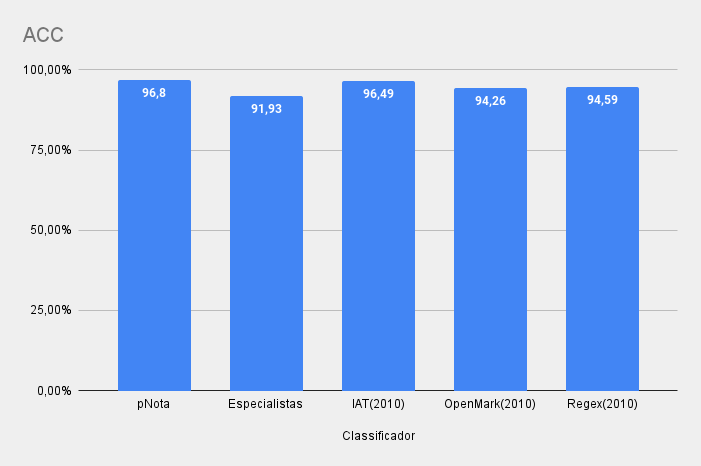
\includegraphics[width=.6\textwidth]{figuras/OU/res-ou-acc.png}
\caption{Resultados obtidos no \textit{dataset} \textit{Open University}.}
\label{fig-OU}
\end{figure}

Na Figura \ref{fig-OU} é demonstrada a alta qualidade da classificação automática em relação ao que foi reportado entre especialistas. Os especialistas atingiram entre eles ACC média de 91,33\%. Os autores \cite{butcher2010} reportaram ACC de 96,49\%. Porém, os três sistemas aplicados utilizam regras e expressões regulares, o que demanda de maior esforço para início das correções. Assim, o sistema deve aguardar enquanto o professor elabora as regras de correção. Como o estudo destaca, o IAT usa o conhecimento sobre o conteúdo e as regras de associação de respostas para criação de \textit{feedbacks} direcionados ao tema.

Outro \textit{dataset} similar é o \textit{Powergrading}. Esse \textit{dataset} também conta com muitas amostras e classificação binária. Foi criado especificamente para estudos que aplicam técnicas de \textit{clusterização} na atribuição de notas \cite{basu2013}. Portanto, uma hipótese é que neste caso há maior separabilidade entre as classes e baixa taxa de sobreposição, algo incomum para respostas discursivas. Consequentemente, o desempenho prévio da clusterização é mais relevante do que a escolha do método de classificação. Os resultados obtidos pelo \textit{p}Nota são apresentados na Tabela \ref{tab-PG}.

\begin{table}
\centering
\caption{Resultados de classificação para o \textit{dataset Powergrading}.}
\label{tab-PG}
\begin{tabular}{l r r r r r}
    \hline
    \multicolumn{4}{l}{\textbf{Powergrading}} & \multicolumn{2}{r}{(2 Categorias)} \\ \hline
     & \multicolumn{5}{c}{M{\'e}tricas} \\ \cline{2-6}

     & ACC & PRE & REC & F1(m) & F1(w) \\ \cline{2-6}
    DTR & 99,79\% & 97,96\% & \textbf{98,68\%} & 98,28\% & 99,80\% \\
    GBC & 99,71\% & 97,46\% & 98,64\% & 97,93\% & 99,74\% \\
    KNN & 99,79\% & 97,96\% & \textbf{98,68\%} & 98,28\% & 99,80\% \\
    RDF & 99,79\% & 97,96\% & \textbf{98,68\%} & 98,28\% & 99,80\% \\
    SVM & \textbf{99,86\%} & \textbf{99,93\%} & 97,50\% & \textbf{98,30\%} & \textbf{99,83\%} \\
    WSD & 99,79\% & 97,96\% & \textbf{98,68\%} & 98,28\% & 99,80\% \\

    \hline
    \hline
\end{tabular}
\end{table}

Como é apontado na Tabela \ref{tab-PG}, alcançamos um bom desempenho com o \textit{p}Nota. Neste, todos os seis classificadores apresentam poucos erros, atingindo ACC de 99,86\% e F1-ponderado de 99,83\%. Nesse caso, o alto desempenho do SVM reforça a hipótese de baixa sobreposição de \textit{features} entre as classes. Os resultados em relação aos demais trabalhos da literatura são apresentados na Figura \ref{fig-PG}.

\begin{figure}[!h]
\centering
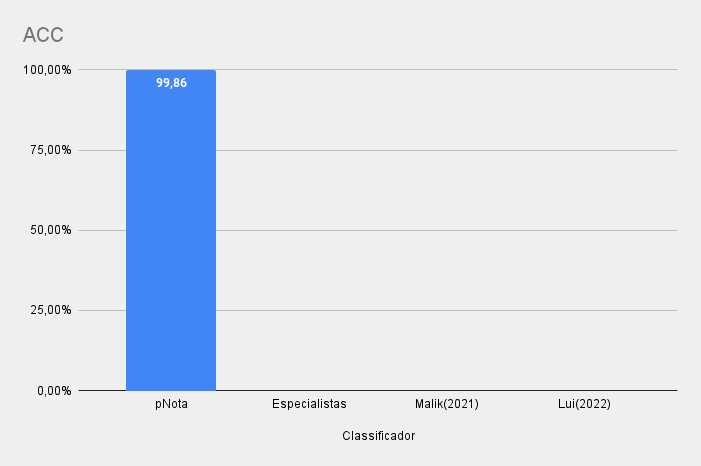
\includegraphics[width=.6\textwidth]{figuras/Powergrading/res-pg-acc.png}
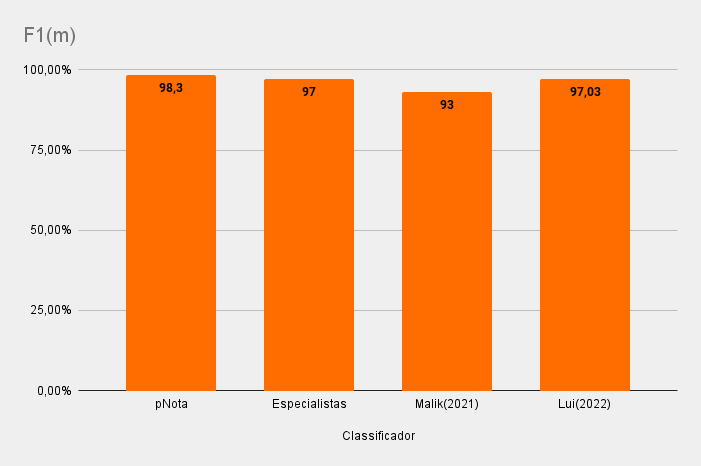
\includegraphics[width=.6\textwidth]{figuras/Powergrading/res-pg-mfs.png}
\caption{Resultados dos classificadores com dados do \textit{dataset} \textit{Powergrading}.}
\label{fig-PG}
\end{figure}

Na Figura \ref{fig-PG} é caracterizada pela alta qualidade obtida na avaliação entre humanos, mas replicada também pelos sistemas. Entre especialistas o F1-macro observado foi de 97\%. O estudo foi realizado por \cite{malik2021}, com foco na formação de \textit{feedbacks} explicativos. Os autores utilizaram DL para elaborar a \textit{Neural Approximate Parsing with Generative Grading} (GG-NAP). Essa técnica visa decompor as respostas para identificar os trechos que compõem uma resposta correta. Entretanto o método não foi feito apenas para respostas discursivas, mas também para atividades com linguagens de programação e programação em blocos. O desempenho como avaliador alcançado é de 93\% de F1-macro. 

Outra proposta foi apontada por \cite{lui2022}, usando \textit{clusterização} e análise de divergências entre as amostras, atingindo F1-macro médio de 97,03\%. O método de \textit{clusterização} aplicado é um \textit{multi-objective evolutionary clustering}, trabalhando os agrupamentos como uma população, buscando o refinamento para aproximar de uma resposta otimizada por \textit{cluster}. A ideia é aumentar a qualidade dos \textit{clusters} segundo suas menções, elegendo sua representação. Portanto, esse conjunto de dados reflete como a etapa de \textit{clusterização} é efetiva para coleta de informações, recuperando a resposta ideal. Entretanto, por mais que ocorram as subpartições entre \textit{clusters} em ambas as propostas, há preocupação com as características que não encontramos no \textit{dataset} \textit{Powergrading}, como altos índices de \textit{outliers} e a \textit{subjetividade} na avaliação.

Seguindo a mesma plataforma avaliativa, o \textit{PTASAG} foi descrito no trabalho de \cite{galhardi2020}. Neste, os autores investigam o impacto das \textit{features} na formação de um bom avaliador. Os níveis estudados foram representação em \textit{n-grams}, representação em \textit{word embeddings}, similaridade léxica, similaridade em \textit{word embeddings}, similaridade em \textit{WordNet} e estatísticas textuais, apresentando nessa ordem maior qualidade. Nessa linha, foram estudadas técnicas primárias (como o tamanho das respostas) até as técnicas consolidadas de \textit{word embeddings} (Word2Vec, GloVe e FastText). O estudo, então, sugere que o maior ganho na avaliação desse \textit{dataset} foi a análise das sequências textuais. O desempenho apresentado pelo \textit{p}Nota é mostrado na Tabela \ref{tab-PTASAG}.

\begin{table}[!h]
\centering
\caption{Resultados de classificação para o \textit{PTASAG}.}
\label{tab-PTASAG}
\begin{tabular}{l r r r r r}
    \hline
    \multicolumn{4}{l}{\textbf{PTASAG}} & \multicolumn{2}{r}{(4 Categorias)} \\ \hline
     & \multicolumn{5}{c}{M{\'e}tricas} \\ \cline{2-6}

     & ACC & PRE & REC & F1(m) & F1(w) \\ \cline{2-6}
    DTR & 88,10\% & 61,39\% & 60,98\% & 60,25\% & 88,01\% \\
    GBC & 90,29\% & 66,14\% & 66,27\% & 64,55\% & 91,07\% \\
    KNN & 87,78\% & 65,77\% & 67,36\% & 64,44\% & 88,46\% \\
    RDF & \textbf{94,49\%} & \textbf{69,04\%} & \textbf{67,98\%} & \textbf{67,32\%} & \textbf{94,05\%} \\
    SVM & 79,13\% & 61,22\% & 61,91\% & 56,55\% & 78,61\% \\
    WSD & 86,33\% & 61,83\% & 62,71\% & 60,48\% & 87,60\% \\

    \hline
    \hline
\end{tabular}
\end{table}

Na Tabela \ref{tab-PTASAG} é mostrado o desempenho da nossa proposta de SAG. Os resultados obtidos expõe o alto desempenho com RDF. Nossa técnica atingiu ACC e F1-ponderado de 94,49\% e 94,05\% respectivamente. Comparando com os níveis de F1-macro, é possível identificar que existe um grande desbalanceamento entre os quatro níveis de nota. Assim, o maior desafio encontrado nesse \textit{dataset} é aprender a avaliar as categorias com amostragem desbalanceada. Os resultados em relação a outros trabalhos da literatura são apresentados na Figura \ref{fig-PTASAG}.

\begin{figure}[!h]
\centering
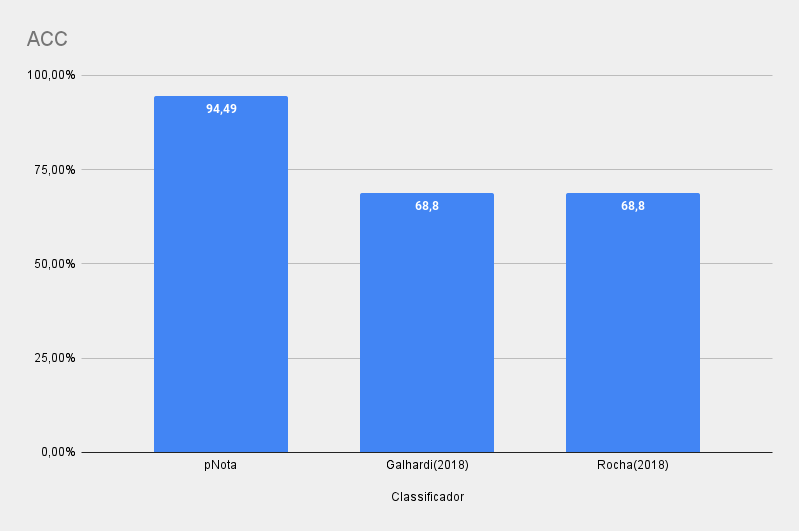
\includegraphics[width=.6\textwidth]{figuras/PTASAG/res-ptasag-acc.png}
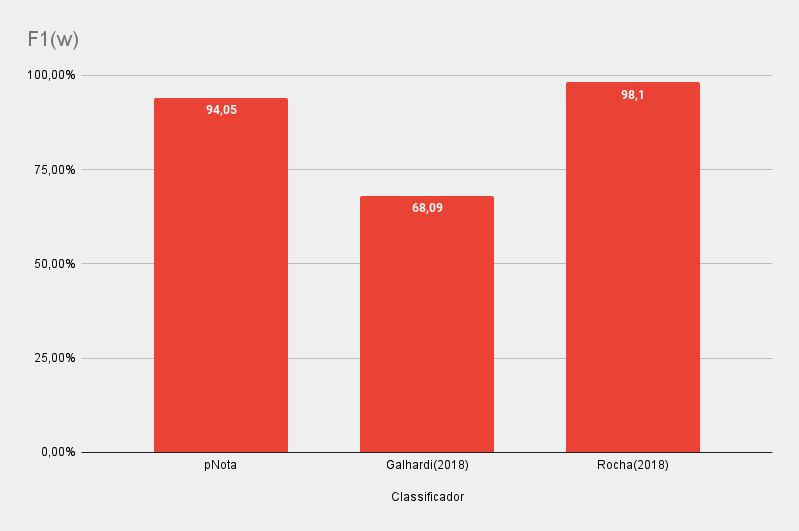
\includegraphics[width=.6\textwidth]{figuras/PTASAG/res-ptasag-wfs.png}
\caption{Resultados dos classificadores com dados do \textit{dataset} \textit{PTASAG}.}
\label{fig-PTASAG}
\end{figure}

Ainda com poucos trabalhos na literatura, na Figura \ref{fig-PTASAG} é mostrado o desempenho dos estudos realizados no \textit{dataset} \textit{PTASAG}. Nesse estudo, os autores reportaram ACC média de 68,8\% e F1-ponderado de 68,09\% com a técnica aqui mencionada \cite{galhardi2018b}. Porém, o ganho obtido com as técnicas de \textit{word-embeddings} não foi reportado nas métricas acima. Ainda assim, segundo o autor, a técnica de \textit{n-grams} apresentou desempenho superior pelo coeficiente \textit{kappa} \cite{galhardi2020}. O coeficiente \textit{kappa} é recomendado para mensurar a equivalência entre pares de avaliadores, entretanto não permite uma comparação justa com diferentes grupos de amostra.

Em um trabalho mais recente, foi estudada a calibração de oito classificadores para este \textit{dataset} \cite{gomes-rocha2021}. Dentre os testes estão os classificadores \textit{Logistic Regression}, \textit{K-Nearest Neighbors}, \textit{Support Vector Machines}, \textit{Bernoulli Naive Bayes}, \textit{Extra Trees}, \textit{Random Forest}, \textit{AdaBoost} e \textit{Multi-layer Perceptron}. \textit{Random Forest} apresentou os melhores resultados com ACC de 68,8\%, mas com ganho marginal em relação a outros classificadores. Os autores também apresentam a F1 e PRE acima de 90\%, mas os resultados aparentam incompatibilidade com a ACC descrita.


Esse processo de avaliação também ocorre com um dos principais \textit{datasets} da literatura. Com origem em uma competição, o \textit{ASAP-SAS} foi criado com partições fixas de treino e teste, com a proposta de avaliação pelo coeficiente \textit{Kappa} quadrático. Os resultados da classificação obtidos pelo \textit{p}Nota são apresentados na Tabela \ref{tab-ASAP-SAS}.


\begin{table}[!h]
\centering
\caption{Resultados de classificação para o \textit{ASAP-SAS}.}
\label{tab-ASAP-SAS}
\begin{tabular}{l r r r r r}
    \hline
    \multicolumn{4}{l}{\textbf{ASAP-SAS}} & \multicolumn{2}{r}{(4 Categorias)} \\ \hline
     & \multicolumn{5}{c}{M{\'e}tricas} \\ \cline{2-6}

    & ACC & PRE & REC & F1(m) &  F1(w) \\ \cline{2-6}
    DTR & 61,03\% & 46,54\% & 47,01\% & 46,39\% & 61,02\% \\
    GBC & \textbf{69,11\%} & \textbf{56,16\%} & \textbf{50,54\%} & \textbf{50,92\%} & \textbf{67,14\%} \\
    KNN & 51,79\% & 38,06\% & 40,36\% & 36,11\% & 52,17\% \\
    RDF & 63,71\% & 51,27\% & 42,19\% & 39,20\% & 57,85\% \\
    SVM & 62,01\% & 44,69\% & 40,29\% & 35,44\% & 54,09\% \\
    WSD & 52,72\% & 44,65\% & 37,39\% & 30,56\% & 48,23\% \\

    \hline
    \hline
\end{tabular}
\end{table}

Na Tabela \ref{tab-ASAP-SAS} é exposto o desempenho de cada um dos classificadores com o \textit{p}Nota. Um destaque é a grande diferença entre as técnicas, caracterizando a formação de sub-espaços complexos para cada nota. Assim, foi encontrada uma diferença de 17,32\% entre GBC e KNN, sendo o primeiro o melhor desempenho com ACC de 69,11\% e F1-ponderado de 67,14\%. Entretanto, para comparar com a literatura foram selecionados os trabalhos que apresentam além do coeficiente \textit{Kappa} o nível de erro encontrado na avaliação, com MAE, MSE e RMSE, mesmo sendo um \textit{dataset} com notas discretas. Assim, o nível de erro apresentado na literatura são descritos na Figura \ref{fig-ASAP-SAS}.

\begin{figure}[!h]
\centering
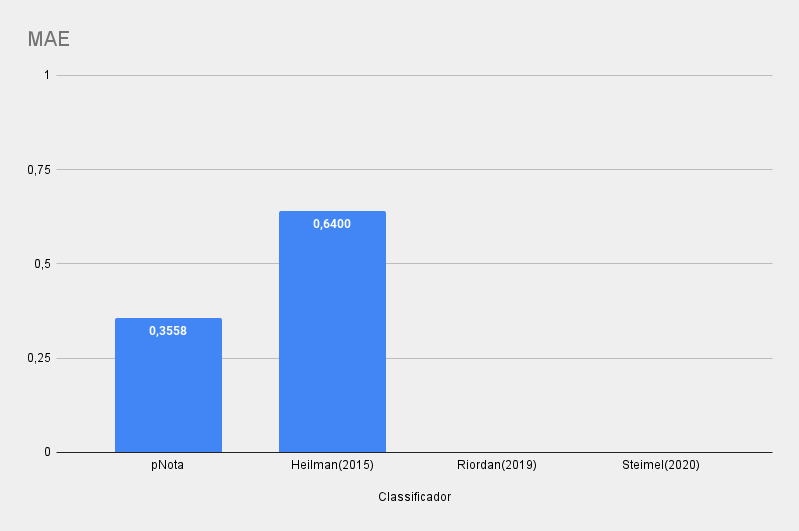
\includegraphics[width=.6\textwidth]{figuras/ASAP/res-asap-mae.png}
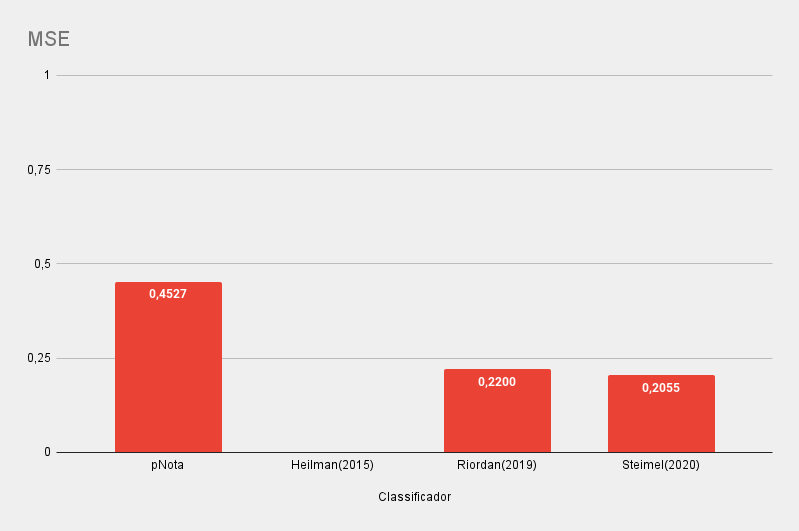
\includegraphics[width=.6\textwidth]{figuras/ASAP/res-asap-mse.png}
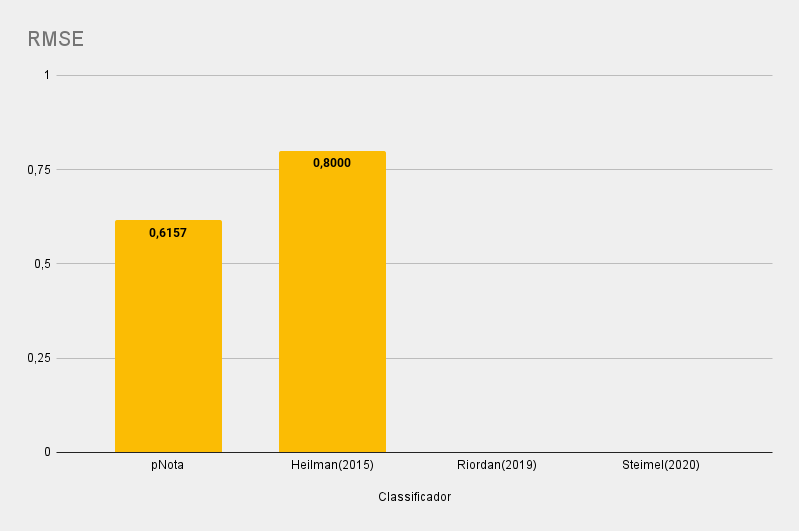
\includegraphics[width=.6\textwidth]{figuras/ASAP/res-asap-rmse.png}
\caption{Resultados dos classificadores com dados do \textit{dataset} \textit{ASAP-SAS}.}
\label{fig-ASAP-SAS}
\end{figure}

Como é destacado na Figura \ref{fig-ASAP-SAS}, o nível de erro apresentado pelo \textit{p}Nota é de 0,3558 pontos de MAE e 0,4527 pontos de MSE. As notas desse \textit{dataset} vão de 0 até 3 pontos. Portanto, o erro resultante leva em conta que não existe gradação entre as quatro classes de nota. O melhor resultado é apresentado por \cite{steimel2020}, com MSE de 0,2055 pontos. Os autores aplicaram DL com \textit{BERT}, uma \textit{bidirectional transformer} com 12 \textit{layers}. A principal mudança aplicada foi o teste de \textit{mean} e \textit{max-pooling} no lugar do padrão aplicado pela rede. Esse trabalho apresenta um ganho interessante em relação ao trabalho anterior dos autores \cite{riordan2019}. Neste primeiro, foi utilizada uma \textit{bidirectional Gated Recurrent Unit}, pré-treinada em uma \textit{word-embeddings}. O principal diferencial desse estudo é a combinação de representações dos documentos (palavras e caracteres) em \textit{Multilayer Perceptron Attention}.

Outro trabalho realizado foi apresentado por \cite{heilman2015}. Nesse estudo foi aplicado \textit{Support Vector Regression}, combinando estruturas sintáticas e semânticas. Para entender a influência de algumas respostas no treinamento, foram replicadas as amostras como forma de reforço. No entanto, os resultados obtidos indicam MAE de 0,64 pontos e um RMSE de 0,80 pontos.

Na mesma linha das avaliações contínuas também há o \textit{dataset} da \textit{University of North Texas}. Esse \textit{dataset} é bem diferente, com apenas 30 respostas por questão. Cada questão foi avaliada por dois avaliadores, \textit{Avaliador1} e \textit{Avaliador2}, em notas de 0 a 5 discretas. Porém, o objetivo é minimizar o erro para a \textit{Média} extraída entre eles. Na Tabela \ref{tab-UNT} são detalhados os resultados obtidos via técnicas de regressão para cada uma das três avaliações.


\begin{table}[!h]
\centering
\caption{Índices de erro obtidos em cada um dos cenários de avaliação do \textit{dataset} da \textit{University of North Texas}.}
\label{tab-UNT}
\begin{tabular}{p{5cm} r r r }
    \hline
    \multicolumn{3}{l}{\textbf{University of North Texas}} & (Notas 0 - 5) \\ \hline
     & \multicolumn{3}{c}{M{\'e}tricas} \\

    & \multicolumn{3}{l}{Avaliador1} \\ \cline{2-4}
     & MAE & MSE & RMSE \\
    LINR & 1,0066 & \textbf{2,5069} & \textbf{1,1955} \\
    LSSR & 1,3273 & 3,1713 & 1,4712 \\
    KNRG & 0,9366 & 2,9032 & 1,2557 \\
    DTRG & \textbf{0,9233} & 3,7338 & 1,4482 \\
    WSRG & 1,2832 & 3,0113 & 1,4240 \\
    \\
    & \multicolumn{3}{l}{Avaliador2} \\ \cline{2-4}
     & MAE & MSE & RMSE \\
    LINR & \textbf{0,4752} & \textbf{0,6099} & \textbf{0,6119} \\
    LSSR & 0,6502 & 0,8605 & 0,7640 \\
    KNRG & 0,4917 & 0,7550 & 0,6658 \\
    DTRG & 0,5121 & 1,2002 & 0,7856 \\
    WSRG & 0,6523 & 0,8839 & 0,7680 \\
    \\
    & \multicolumn{3}{l}{Média} \\ \cline{2-4}
     & MAE & MSE & RMSE \\
    LINR & \textbf{0,5058} & \textbf{0,5476} & \textbf{0,6199} \\
    LSSR & 0,7299 & 0,8464 & 0,8170 \\
    KNRG & 0,5055 & 0,6804 & 0,6765 \\
    DTRG & 0,5811 & 1,1244 & 0,8372 \\
    WSRG & 0,7024 & 0,8088 & 0,7920 \\

    \hline
    \hline
\end{tabular}
\end{table}

Na Tabela \ref{tab-UNT} é apresentado o nível de erro para cada avaliação, com destaque para a \textit{Média}. O \textit{p}Nota apresenta MAE de 0,5058, MSE de 0,5476 e RMSE de 0,6199 pontos. Por conta dessa baixa quantidade de amostras, há um problema na comparação com os demais estudos da literatura. Alguns métodos utilizam até 12-\textit{Fold} durante a avaliação \cite{kumar2017, saha2018}. No caso do \textit{p}Nota, com treino fixado pelo método de \textit{clusterização}. Porém, foi designado 75\% das amostras para treinamento tal qual encontrado em outros \textit{datasets} da literatura.

\begin{figure}[!h]
\centering
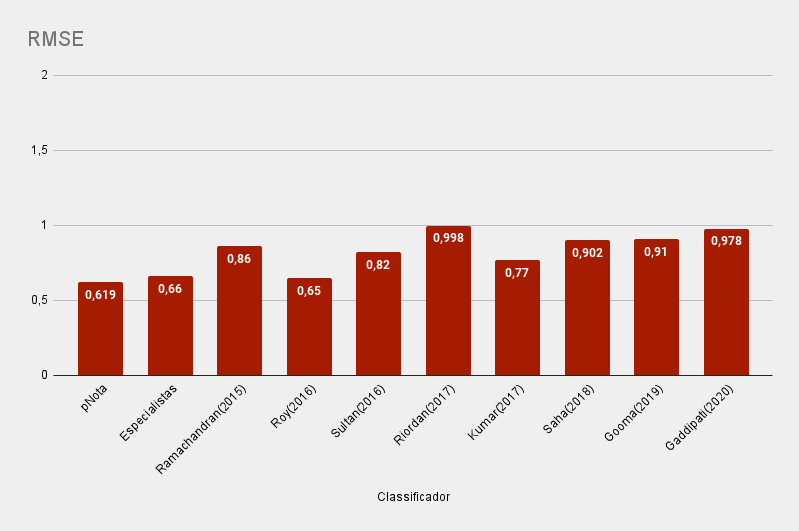
\includegraphics[width=.6\textwidth]{figuras/UNT/res-unt-rmse.png}
\caption{Resultados dos avaliadores com dados do \textit{dataset} \textit{University of North Texas}.}
\label{fig-UNT}
\end{figure}


Na Figura \ref{fig-UNT} é mostrado um detalhe interessante na evolução dos sistemas SAG. Os sistemas mais recentes, em ordem da esquerda para a direita, aumentaram consideravelmente o erro nesse \textit{dataset}. Nesse cenário, o menor erro encontrado foi obtido pelo \textit{p}Nota, com apenas 0,619 pontos de RMSE para a média dos avaliadores. Isso acontece com os métodos já descritos \cite{riordan2017, saha2018, gomaa2019, ramachandran2015b}. 

A divergência observada entre os especilistas nesse \textit{dataset} foi de 0,66 pontos. Apenas o trabalho descrito por \cite{roy2016} chegou a esse nível, com RMSE de 0,65 pontos. Seu diferencial, como comentado anteriormente, foi uma métrica de sobreposição entre respostas, calculando equivalência e divergências entre as respostas. Em um trabalho mais elaborado, \cite{kumar2017} atingiu 0,77 pontos de RMSE com uma técnica específica de \textit{pooling} aplicada em \textit{Siamese LSTMs}. Para reforço do aprendizado com poucas amostras, os autores utilizaram \textit{data aumentation}. Enquanto uma LSTM trabalha no \textit{encodding} da resposta candidata, a segunda realiza o \textit{encodding} das respostas dos alunos. O \textit{layer} que avalia a compatibilidade utiliza a \textit{Earth mover distance pooling}. Essa distância calcula a transferência mínima para aproximar os dois vetores na comparação de sequencias em \textit{word embeddings}.

O trabalho mais recente de \cite{gaddipati2020} mostra uma comparação do desempenho de modelos de \textit{Transfer Learning}. Entre eles há o ELMo, GPT, GPT-2 e BERT. Os autores utilizaram 70\% dos dados para treino e 30\% para teste. Os autores compararam os resultados com outros métodos de análise vetorial tradicionais como TF-IDF, \textit{Word2Vec}, \textit{GloVe} e \textit{FastText}. O melhor resultado obtido foi com o ELMO, com 0,978 pontos de RMSE. Ainda nesse estudo os autores destacam o problema do desbalanceamento das notas, com média de 4,17 pontos por resposta, tornando bem complexa a tarefa de aprendizado para níveis menores de nota.

Outros dois \textit{datasets} aplicados foram com dados locais. O \textit{dataset} \textit{VestUFES} foi utilizado durante os anos para o desenvolvimento do \textit{p}Nota \cite{spalenza2017}. O primeiro é aplicado com dados do vestibular da universidade. Ele contém notas normalizadas para a escala de 0 a 10, mas foi avaliador inicialmente em notas contínuas entre 0 e 2 pontos. Os resultados de avaliação do \textit{p}Nota são apresentados na Tabela \ref{tab-VEST}.

\begin{table}[!h]
\centering
\caption{Índices de erro obtidos em cada um dos cenários de avaliação do \textit{dataset} do \textit{VestUFES}.}
\label{tab-VEST}
\begin{tabular}{p{5cm} r r r }
    \hline
    \multicolumn{3}{l}{\textbf{VestUFES}} & (Notas 0 - 10) \\ \hline
     & \multicolumn{3}{c}{M{\'e}tricas} \\

    & \multicolumn{3}{l}{Avaliador1} \\ \cline{2-4}
     & MAE & MSE & RMSE \\
    LINR & 1,8614 & \textbf{6,0562} & \textbf{2,3261} \\
    LSSR & 2,4570 & 9,5859 & 2,9596 \\
    KNRG & 1,9058 & 6,8529 & 2,5057 \\
    DTRG & \textbf{1,6348} & 7,0130 & 2,5333 \\
    WSRG & 2,4665 & 9,6489 & 2,9515 \\
    \\
    & \multicolumn{3}{l}{Avaliador2} \\ \cline{2-4}
     & MAE & MSE & RMSE \\
    LINR & 1,7943 & \textbf{5,2526} & \textbf{2,1898} \\
    LSSR & 2,4358 & 8,5399 & 2,8264 \\
    KNRG & 1,7290 & 6,3471 & 2,3781 \\
    DTRG & \textbf{1,6783} & 7,7696 & 2,6739 \\
    WSRG & 2,4282 & 8,5112 & 2,8111 \\

    & \multicolumn{3}{l}{Final} \\ \cline{2-4}
     & MAE & MSE & RMSE \\
    LINR & 1,8556 & \textbf{5,4816} & \textbf{2,2326} \\
    LSSR & 2,5365 & 9,5175 & 2,9435 \\
    KNRG & \textbf{1,7667} & 6,7042 & 2,3789 \\
    DTRG & 1,8457 & 8,3614 & 2,6566 \\
    WSRG & 2,5256 & 9,4779 & 2,9198 \\

    \hline
    \hline
\end{tabular}
\end{table}

Na Tabela \ref{tab-VEST} são mostrados resultados distintos entre as notas individuais dos avaliadores e o resultado médio. Tanto para o \textit{Avaliador 1} quanto para o \textit{Avaliador 2}, o menor nível de erro observado em MAE foi dado pelo DTRG. No entanto, para a nota média o KNRG apresentou melhor desempenho com MAE de 1,7667 pontos.

O segundo \textit{dataset} local foi desenvolvido em 2019 para retratar um pouco melhor os resultados em dados nacionais. O \textit{dataset} do \textit{Projeto Feira Literária} foi coletado em conjunto com os autores para descrição da aplicação do \textit{p}Nota e seu uso por professores \cite{nascimento2020}. Este caracteriza-se pela presença de erros de escrita e por conteúdos fora de tópico, sendo fatores avaliados negativamente pelo tutor. Na Tabela \ref{tab-FINDES} é apresentado o desempenho de cada um dos seis classificadores e seus resultados alcançados na avaliação das questões do projeto.


\begin{table}[!h]
\centering
\caption{Resultados de classificação para o \textit{Projeto Feira Literária}.}
\label{tab-FINDES}
\begin{tabular}{l r r r r r}
    \hline
    \multicolumn{4}{l}{\textbf{Projeto Feira Literária}} & \multicolumn{2}{r}{(4 Categorias)} \\ \hline
     & \multicolumn{5}{c}{M{\'e}tricas} \\ \cline{2-6}

     & ACC & PRE & REC & F1(m) & F1(w) \\ \cline{2-6}
    DTR & 77,86\% & 59,99\% & 59,29\% & 58,42\% & 76,84\% \\
    GBC & \textbf{78,58\%} & 59,58\% & 59,57\% & 57,07\% & \textbf{77,74\%} \\ 
    KNN & 65,00\% & 58,72\% & 58,02\% & 54,75\% & 66,91\% \\
    RDF & 78,57\% & \textbf{61,82\%} & \textbf{64,98\%} & \textbf{61,36\%} & 76,53\% \\
    SVM & 72,86\% & 51,49\% & 57,85\% & 49,34\% & 67,66\% \\
    WSD & 75,71\% & 54,77\% & 61,24\% & 56,14\% & 74,57\% \\

    \hline
    \hline
\end{tabular}
\end{table}

Conforme é caracterizado na Tabela \ref{tab-FINDES}, há alta qualidade de três classificadores RDF, DTR e GBC. O último, em especial, teve o maior desempenho com 78,58\% de ACC. Com 70 respostas e a pluralidade de estruturas textuais encontradas, destaca-se a semelhança deste \textit{dataset} com os desafios apresentados por \textit{Beetle} e \textit{SciEntsBank} no ensino de ciências.

\section{Discussão de Resultados}
\label{sec-discussao}

A avaliação de questões discursivas é uma área que evoluiu muito em relação as propostas iniciais dos anos 60. O volume de dados e a capacidade de processamento e suporte computacional foram fundamentais para incorporar isso na rotina avaliativa do professor. Dos sistemas mais rígidos, que operam com regras e padrões pré-fixados, até hoje com maior profundidade dos modelos com análises de NLP. Isso inclui técnicas de ML e DL aparecendo nos trabalhos mais recentes.


O volume limitado de amostras por tema, enunciado e nota são contrastantes com os requisitos e a autonomia de técnicas mais robustas de classificação. Para isso, muitos métodos consideram o \textit{dataset} como um todo para treinamento, agrupando toda série de atividades para compreender, em nível macro, cada nível de nota. Isso inibe parcialmente a falta de amostras mas presume \textit{a priori} uma equivalência contextual. Essa equivalência nem sempre existe. Certas situações podem afetar diretamente a produção textual que, se não analisadas separadamente, causam problemas na interpretação entre a equivalência e divergência contextual. Isolando essas situações, podemos identificar alterações em notas, experiências, plágios e cenários avaliativos. 

Uma situação que pode causar isso é a aplicação de uma questão com turmas que tiveram experiências distintas. Se uma turma teve contato com um objeto da questão enquanto outra não teve, possivelmente temos impacto direto na forma de resposta. Quando tal situação é explorada nas atividades disponibilizadas pelo professor, esse tipo de situação ganha ainda mais notoriedade.

Por conta disso, os estudos do \textit{p}Nota envolvem comprender os diferentes relatos dos estudantes para assimilar detalhes sobre o contexto. Então, mesmo nesse caso, presume-se a coerência e a consistência textual, mas apenas em no nível das atividades. É interessante a partir daí, que ocorra o enriquecimento textual. Por isso, os trabalhos mais recentes combinam várias formas de interpretação do texto, atingindo ao menos níveis semânticos e sintáticos.

Assim, na criação do modelo linguístico, de uma forma geral os sistemas trabalham o alinhamento entre o conjunto de respostas e as respostas candidatas. A proposta apresentada neste trabalho busca iterações com o professor para evolução do modelo criado. Para além da análise textual o sistema prioriza a conexão entre conteúdo e critério avaliativo. Dessa maneira, as nuances do contexto são interpretadas pelo tutor durante a avaliação, destacada com o critério de atribuição de notas. Superdimensionados para a avaliação de uma determinada disciplina ou tema, os modelos rígidos divergem bastante da aplicação dos sistemas SAG no cotidiano do professor. Assim, o professor espera que o sistema seja capaz de reduzir o esforço de correção, dando suporte ao seu método assim que requisitado. Independentemente do cenário ao qual é aplicado, o sistema SAG deve lidar com as respostas como parte do ensino-aprendizagem, buscando minorar a demanda de verificação do conteúdo.

De qualquer forma, pela dinâmica dos trabalhos na área, vê-se que é muito complexa a tarefa de se adequar a todos os cenários. Nessa perspectiva, é identificado com o \textit{p}Nota um ótimo desempenho nos diferentes \textit{datasets}, sendo equiparável aos resultados da literatura em todos os testes. Além disso, o vínculo do método avaliativo com as características textuais encontradas no \textit{p}Nota tem maior capacidade de resolver questões do que boa parte dos sistemas mencionados. Isso acontece porque a proposta aqui descrita busca compreender diferenças encontradas nos dados antes do processo avaliativo. De forma geral, a preocupação com a modelagem do critério avaliativo torna mais efetiva a contextualização sobre o tema. Consequentemente, um sistema contextualizado tende a apresentar bom desempenho como avaliador.

O \textit{p}Nota também precisa de apenas algo entre seis minutos e uma hora para processamento em um computador comum. Essa variação é dada especificamente pelo número de testes executados, vinculado principalmente às características de cada atividade. Essa \textit{performance} foi observada em um computador com processador Intel Core i7-8700 (3,2GHz x 12) com 16 GB de memória, portando uma placa de vídeo NVIDIA GeForce GTX 1070. O tempo de execução é definido segundo o número de etapas e o número de características encontradas nas amostras do conjunto de dados. Esse tempo é resultado de um refinamento dos processos e redução de testes que não adicionavam valor aos processos. Porém, essa avaliação considera apenas o tempo do sistema, desconsiderando as interações e o tempo de anotação com o professor durante a execução. Apesar de enquadrar-se bem no tempo que o professor demanda para avaliar cada uma das respostas, ainda são válidos os esforços para otimizar as etapas parciais de cada um dos processos para a melhoria da \textit{performance} geral. Logo, esse tipo de sistema deve atender ao problema e, simultaneamente, ser associado à rotina de avaliação do professor.

Ainda é importante salientar que, entre todas as comparações criadas com os \textit{datasets} disponíveis, o modelo proposto neste trabalho foi o mesmo aplicado para todas as questões. Os processos de otimização que compõe o modelo que realizam a calibração do que deve ser entregue ao professor. Portanto, o \textit{p}Nota não aprensenta rigidez e contextualização que são necessários a parte dos modelos que atuam em domínios específicos. Assim, inclui-se na qualidade dos resultados obtidos a capacidade do próprio sistema de adaptação ao tema e ao modelo de avaliação, sendo parte das etapas do \textit{p}Nota a calibração dos processos.

A escolha dos modelos é realizada pela paridade com os resultados obtidos nas amostras com avaliação do especialista. Por conta disso, o \textit{p}Nota conta com flexibilidade para estudar o contexto aplicado a cada questão e otimizar o aprendizado dos algoritmos. A tendência, então, é que os métodos selecionados apresentem o melhor reconhecimento dos grupos de nota, seja via técnicas de classificação ou de regressão.

Por fim, para avaliar os resultados obtidos com tal processo de classificação, foi testada a hipótese de que o classificador GBC apresenta resutados superiores, dado que o mesmo mostrou-se melhor na maioria dos cenários. Para isso, o primeiro teste realizado foi o Teste de Shapiro-Wilk, onde é avaliado se os resultados seguem ou não uma distribuição normal. A normalidade da distribuição foi rejeitada com \textit{p-value} de 0.0038. Um segundo teste, Teste de Levene, foi aplicado para verificar se os resultados apresentam variâncias iguais. Com um \textit{p-value} de 0.9419 os resultados mostram que as amostras são homogêneas, sem diferenças significativas entre as variâncias. Por fim, o terceito teste aplicado foi o Teste de Kruskal-Wallis, onde foi avaliado se, dado a homogeniedade da variância, as amostras têm origem em uma mesma distribuição. Entretanto, a não-rejeição da hipótese corrobora com as principais contribuições deste trabalho. Mesmo não apresentando uma diferença significativa nos métodos de classificação, o ganho em relação aos métodos da literatura é obtido via \textit{Active Learning}, dado o ciclo completo do \textit{p}Nota.
